% \setchapterimage[6cm]{seaside}
\setchapterpreamble[u]{\margintoc}
% \chapter{Defining a model of the implicit object construction}
\chapter{A Stochastic Optimality Theoretic account of object drop}
\labch{modeltheory}


\section{Optimality Theories} \labsec{introtheory}

The model of the implicit object construction presented in this dissertation was developed under the Optimality Theory framework. In particular, it builds on the specific flavor of Stochastic Optimality Theory defined by \textcite{Medina2007} in order to model object drop in English.\\
In \refsec{classicot} I will present standard Optimality Theory and discuss both its strengths and its shortcomings. \refsec{harmonic_grammar} is devoted to Harmonic Grammar, the historical precursor of Optimality Theory, which is shown to possess attractive mathematical properties its descendant lacks, but also a number of problems making it a bad fit for modeling object drop. In \refsec{otgradience} I tackle the problem of moving from modeling the binary judgments traditionally used in syntax theory to modeling complex gradient judgments, which leads to the development of probabilistic grammars. A discussion of these and an in-depth introduction to Stochastic Optimality Theory are provided in \refsec{stochot}.

\subsection{Optimality Theory} \labsec{classicot}

\paragraph{Introduction} In \nrefch{factors}, the optionality of direct objects has been shown to depend on a large number of semantic, aspectual, and pragmatic factors. The challenge a linguistic model of object drop has to undertake is to account not only for the existence of relevant factors, but also for their combined effect on the grammaticality of the implicit object construction. My model will be based upon a probabilistic variant of Optimality Theory \parencite{princesmolensky1993optimality, PrinceSmolensky2008}. A full introduction to Optimality Theory and its intricacies goes well beyond the scope of this thesis, so I will only provide a short presentation to familiarize the reader with the framework and clarify its role in my research.\\ % 1. OPTIMALITY THEORY FOUNDATIONS
In a nutshell, the grammaticality of a linguistic structure in Optimality Theory is defined in terms of well-formedness with respect to a set of conflicting, re-rankable constraints. The constraints themselves are universal, while the order in which they are ranked is language-specific and determines the optimal (i.e. grammatical) output. How does this work in practice? Let us look at an example of the basic workings of Optimality Theory by \textcite{grimshaw1998optimal}, made classic in the introduction to the use of the framework in syntactic theory by \textcite{legendre2001introduction}, and finally revised in \textcite{legendre2019otsyntax}. The version of the linguistic examples and of the constraints discussed here is the latest one by \textcite{legendre2019otsyntax}.\\
A linguistic phenomenon often mentioned in textbooks is that languages allowing for topic-referring subjects to be dropped also require null expletives with weather verbs (as in \ref{ita_nullsubj}), while languages with compulsorily overt subjects require overt expletives with weather verbs (as in \ref{eng_nullsubj}).
\ex. \label{ita_nullsubj} Italian
\a. (Ha) mangiato tre panini.
\b. \label{ita_expletive} (*Esso) piove.

\ex. \label{eng_nullsubj} English
\a. *(She) has eaten three burgers.
\b. \label{eng_expletive} *(It) rains.

% COMPACT EXAMPLES AS IN https://www.ling.upenn.edu/~beatrice/syntax-textbook/glossary.html
In order to account for the difference between Italian and English with respect to their treatment of expletives, as shown in \ref{ita_expletive} and \ref{eng_expletive} respectively, the Optimality Theoretician has to individuate the relevant constraints and to set a conflict between them, i.e. to define them so that satisfying a constraint entails a violation of another.\\
% FAITHFULNESS/MARKEDNESS CONSTRAINTS
In this case, only the two constraints in \ref{expletive_constraints} are at play. In particular, \textsc{Subject} \ref{expletive_subj} is the re-working of the Extended Projection Principle \parencite{chomsky1982epp} as a markedness constraint, while \textsc{Full-Int} \ref{expletive_fullint} is a faithfulness constraint capturing the Principle of Full Interpretation \parencite{chomsky1991fullint}.
\ex. \label{expletive_constraints} \a. \label{expletive_subj} \textsc{Subject}: The subject surfaces in SpecTP.
\b. \label{expletive_fullint} \textsc{Full-Int}(erpretation): Lexical items contribute to the interpretation of a structure.

\textsc{Subject} and \textsc{Full-Int} are in conflict in the case of zero-argument verbs (such as weather verbs) because satisfying the former requires the use of an overt expletive, which is forbidden by the latter, while satisfying \textsc{Full-Int} requires a null expletive, which goes against \textsc{Subject}. No sentence can possibly satisfy both constraints at the same time. Conflicts in Optimality Theory are solved by re-ranking the constraints based on the violations each competing candidate incurs into.\\
Let us discuss the tableaux for Italian and English weather verbs, in \reftab{tableau_ita_expletive} and \reftab{tableau_eng_expletive} respectively, where the competition between candidates and its outcome are made esplicit.

\begin{table}[htb] % the "htb" makes table env unfloaty
\caption{Optimality Theoretic tableau for weather verbs in Italian.}
\labtab{tableau_ita_expletive}
\begin{tabular}{|ll|c|c|}\hline   
      & \textbf{\textit{piovere}\textsubscript{v}[present]}  & \textsc{Full-Int}  &  \textsc{Subject}\\ \hline\hline
      & a. EXPL piove     & *!         &           \\ \hline
\hand & b. piove     &            & *       \\ \hline
\end{tabular}
\end{table}

\begin{table}[htb] % the "htb" makes table env unfloaty
\caption{Optimality Theoretic tableau for weather verbs in English.}
\labtab{tableau_eng_expletive}
\begin{tabular}{|ll|c|c|}\hline   
      & \textbf{\textit{rain}\textsubscript{v}[present]}  & \textsc{Subject}  &  \textsc{Full-Int}\\ \hline\hline
\hand      & a. EXPL rains     &           & *         \\ \hline
 & b. rains     & *!           &       \\ \hline
\end{tabular}
\end{table}

The input to syntactic optimization in Optimality Theory contains only the relevant semantic information (lexical items, argument structures, and tense specifications), and all competitors share the same semantic content. In our case, the input contains the verb, its tense, and no argument structure since weather verb have no thematic arguments. Crucially, the expletive subject is not part of the input. Instead, it is supplied to a candidate output by \textsc{Gen}, the Generator function mapping the input to the set of all possible candidates to the optimization. The resulting set comprises two candidates, one with an expletive subject (in $a.$) and one without (in $b.$). As explained above, candidates with an expletive subject violate \textsc{Full-Int} and subject-less candidates violate \textsc{Subject}. In the tableaux, an asterisk marks a violation of a constraint, an exclamation mark after an asterisk marks a \textit{fatal} violation (i.e. a violation excluding the candidate from further evaluation), the pointing finger indicates the optimal candidate, and constraints are ordered so that each constraint dominates the one to its right. Given the typology sketched in \ref{ita_expletive} and \ref{eng_expletive}, an Optimality Theoretic analysis of Italian and English leads to the conclusion that the difference between the two languages with respect to zero-argument verbs results from the different ranking of two universal constraints, \textsc{Full-Int} and \textsc{Subject} (as shown in the tableaux  \reftab{tableau_ita_expletive} and \reftab{tableau_eng_expletive}).\\
An explanation of the behavior of weather verbs in Italian and English, as well as a broader account of the typology in \ref{ita_nullsubj} and \ref{eng_nullsubj}, is not something that can happen only under Optimality Theory. For instance, Principles-and-Parameters theory accounts for the different behavior of Italian and English with the \textsc{Pro-Drop} parameter, so that Italian is a [+pro-drop] language and English is a [-pro-drop] language. In such a framework, inviolable, fixed parameters determine the grammaticality of a linguistic structure in a given language. Optimality Theory on the contrary, as "a formal theory of constraint interaction in Universal Grammar" \parencite{legendre2001introduction} relies on violable, re-rankable constraints to determine grammaticality. Most importantly, grammaticality is given to a linguistic structure as the outcome of a competition among several candidates, instead of being a property of that linguistic structure taken on its own. This is a crucial aspect of Optimality Theory that makes it a suitable framework for my analysis of the implicit object construction, even though \textit{standard} Optimality Theory suffers from problems that are best solved by other variants of the same framework. % 5. Kuhn's examples against standard OT
\paragraph{Impossible violation profiles} To explain the nature of these problems, I will start with an example. Let us say that we collected a small set of data from a single language, that we wanted to model the distribution of these data using three theory-driven constraints, and that these data presented the constraint violation profiles represented in \reftab{tableau_kuhn_1}, \reftab{tableau_kuhn_2}, and \reftab{tableau_kuhn_3}.

\begin{table}[htb] % the "htb" makes table env unfloaty
\caption{Hypothetical Optimality Theoretic tableau for mock data by \textcite{kuhn2002corpus}}
\labtab{tableau_kuhn_1}
\begin{tabular}{|ll|c|c|c|}\hline   
      & \textbf{(a) candidate set:}  & \textsc{Constr. 3}  &  \textsc{Constr. 1} & \textsc{Constr. 2}\\ \hline\hline
\hand      & candidate A     &           & *         & * \\ \hline
 & candidate B     & ***           &       & \\ \hline
\end{tabular}
\end{table}

\begin{table}[htb] % the "htb" makes table env unfloaty
\caption{Hypothetical Optimality Theoretic tableau for mock data by \textcite{kuhn2002corpus}}
\labtab{tableau_kuhn_2}
\begin{tabular}{|ll|c|c|c|}\hline   
      & \textbf{(b) candidate set:}  & \textsc{Constr. 1}  &  \textsc{Constr. 2} & \textsc{Constr. 3}\\ \hline\hline
\hand      & candidate A'     &           &          & * \\ \hline
 & candidate B'     &            & *      & \\ \hline
\end{tabular}
\end{table}

\begin{table}[htb] % the "htb" makes table env unfloaty
\caption{Hypothetical Optimality Theoretic tableau for mock data by \textcite{kuhn2002corpus}}
\labtab{tableau_kuhn_3}
\begin{tabular}{|ll|c|c|c|}\hline   
      & \textbf{(c) candidate set:}  & \textsc{Constr. 1}  &  \textsc{Constr. 2} & \textsc{Constr. 3}\\ \hline\hline
\hand      & candidate A''     &           &          & * \\ \hline
 & candidate B''     & *           &       & \\ \hline
\end{tabular}
\end{table}

It is evident that this model of our mock data is unfeasible, considered that in any given language the constraints have to be ordered consistently (under the assumption of strict dominance). However, in the model above this does not happen, since \reftab{tableau_kuhn_1} is a ranking argument for \textsc{Constr. 3} $\gg$ \textsc{Constr. 1} and \textsc{Constr. 3} $\gg$ \textsc{Constr. 2}, while \reftab{tableau_kuhn_2} and \reftab{tableau_kuhn_3} are ranking arguments for the opposite.\\
It's possible that these constraints have to be ditched in favor of a whole new set of constraints, in theory, but let's say they are very well motivated by literature on the topic and there is no reason in linguistic theory to doubt their effect on the grammaticality of these data. Another possible solution to the inconsistency would be to introduce an additional constraint, \textsc{Constr. 4}, which would be ranked higher than all the others and violated only by candidate B. Provided we could indeed find such a constraint, this would lead to a situation where all the candidate sets from this hypothetical language are consistent with the ordinal constraint ranking \textsc{Constr. 4} $\gg$ \textsc{Constr. 1} $\gg$ \textsc{Constr. 2} $\gg$ \textsc{Constr. 3}. Yet, \textsc{Constr. 4} may be weakly grounded in the linguistic theory and thus a poor choice for a constraint in an Optimality Theoretic analysis. Remember that constraints are assumed to be part of Universal Grammar, and they have to be ranked consistently within a given language. What if \textsc{Constr. 4} is found to be incompatible with newer data from the same hypothetical language considered above? The quest to find an additional suitable constraint could continue, but the same problem would resurface again and lead to an unmotivated number of constraints very quickly. I will provide a possible solution to this problem (and discuss its shortcomings) in \refsec{harmonic_grammar}. % 2. OT RELIES ON BINARY JUDGMENTS AND THEY ARE BAD FOR OBJ DROP
\paragraph{Why standard OT is a bad fit for a model of object drop} \labpage{ot_bad_dobjdrop}
I will now focus on a feature of standard Optimality Theory that, while not being a worrying issue \textit{per se}, may become a problem for those using it to model a phenomenon as complex as the indefinite object constructions. Let us see why.\\
Linguists adopting standard Optimality Theory to perform their analyses of syntax and other aspects of grammar rely on binary grammaticality judgments. As illustrated above, given a set of candidates competing for optimality, the optimization yields only one optimal candidate, which is the only deemed grammatical, while all the others are equally ungrammatical regardless of the number or ranking of constraint violations they incurred into. Now, considering the phenomenon examined in this dissertation, a traditional Optimality Theoretic approach to modeling the grammaticality of the implicit object construction would only account for an oversimplified typology such as the one in \ref{naive_objdrop}. 
\ex. \label{naive_objdrop} \a. \label{naive_objdrop_sing} John sang.
\b. \label{naive_objdrop_build} *John built.

Such an account would perfectly describe a world where the linguistic factors presented in \nrefch{factors} make some object-less sentences with transitive verbs fully grammatical (as in \ref{naive_objdrop_sing}) and other ones fully ungrammatical (as in \ref{naive_objdrop_build}). However, the actual scenario is more complex. For instance, a classic Optimality Theoretic analysis of object drop would not capture the different grammaticality of the sentences in \ref{mature_objdrop_eat}, even though the literature suggests the imperfective sentence should be at least slightly more acceptable than the sentence in the perfective aspect. Similarly, it would fail to model cases such as \ref{mature_objdrop_build}, where neither candidate is fully grammatical, making it weird, if not altogether wrong, to declare an \textit{optimal} candidate.
\ex. \label{mature_objdrop_eat} \a. John had eaten.
\b. John was eating.

\ex. \label{mature_objdrop_build} \a. *John built.
\b. \textsuperscript{?}John was building again.

Example \ref{failot_medina} is the one used by \textcite[62]{Medina2007} to make the point that, crucially, the grammaticality of indefinite object drop varies not only within a group of candidates featuring the same verb, but also across verbs.
\ex. \label{failot_medina} \a. Jack ate.
\b. *Jack found.
\c. \textsuperscript{?}Jack caught.

Standard Optimality Theory fails to capture all of these observation in a working model of object drop. I will discuss possible solutions to this problem in \refsec{otgradience} and focus on the one I will use for my experiments in \refsec{stochot}.

\subsection{Harmonic Grammar} \labsec{harmonic_grammar} % 6. Kuhn's examples introducing Harmonic Grammar
Let us forgo standard Optimality Theory and try replacing ranked ordinal constraints with numerically weighted ones, to avoid resorting to additional constraints and solve the problem of having impossible violation profiles. 
This was actually the strategy employed by the historical precursor of Optimality Theory, Harmonic Grammar, sketched out by \textcite{smolensky1993integrating, legendre1990can, legendre1991unifying} and later discussed in the light of Optimality Theory by \textcite{legendre2006optimality, pater2009weighted}. Harmonic Grammar was created as an attempt to bridge the apparently insurmountable gap between generative grammar, which is a formal model of existing languages, and linguistic models based on connectionism, which are instead models of cognition translating the patterns of neural activity into mathematical functions. In practice, Harmonic Grammar models assign a non-negative numerical weight to each constraint, each candidate gets a negative score for each violation of a constraint or a positive score for each satisfaction (unlike in Optimality Theory), and the harmony of each candidate is computed as in \refeq{harmony}. 

\begin{equation} \labeq{harmony} % formula in Pater (2009: 1006)
H = \sum_{k=1}^{K} s\textsubscript{k} w\textsubscript{k}
\end{equation}

Given a set of $k$ constraints, s\textsubscript{k} is the violation score of a candidate and w\textsubscript{k} is the weight of a constraint. The only candidate deemed grammatical, i.e. the winner of the competition for optimality, is the most harmonic in the candidate set. Unlike in Optimality Theory, where strict domination determines that the violation of a higher-ranked constraint is always worse than the violation of a lower-ranked constraint, the weighting of constraints in Harmonic Grammar makes it possible to model the cumulative effect of multiple violations of a constraint (see \reftab{hg_kuhn_1}). Most importantly, there is no notion of constraint \textit{ranking} in Harmonic Grammar, so that their ordered depiction in tableaux has no bearing on the model itself.\\
Let us look at some made-up examples in \reftab{hg_kuhn_1}, \reftab{hg_kuhn_2}, and \reftab{hg_kuhn_3}, adapted from \textcite{kuhn2002corpus} to conform to Harmonic Grammar symbolism. Unlike tableaux in Optimality Theory, Harmonic Grammar tableaux have an additional row for constraint weights and an additional column for the harmony scores of candidates. It appears that the starting weights assigned to the three constraints in the examples below do not determine a reliable model, since they are compatible with the candidate sets (a) and (b), but not with (c), where candidate B results more harmonic than candidate A.

\begin{table}[htb] % the "htb" makes table env unfloaty
\caption{Hypothetical Harmonic Grammar tableau for mock data, adapted from \textcite{kuhn2002corpus}}
\labtab{hg_kuhn_1}
\begin{tabular}{|ll||c|c|c||c|}\hline   
      & \textbf{(a) candidate set:}  & \textsc{\rotatebox[origin=c]{90}{ Constr. 1 }}  &  \textsc{\rotatebox[origin=c]{90}{ Constr. 2 }} & \textsc{\rotatebox[origin=c]{90}{ Constr. 3 }} & \textit{H}\\
       &  & 4 & 3 & 1 & \\
      \hline\hline
\hand      & candidate A     & -1          &          & -1 & -5 \\ \hline
 & candidate B     &            & -3      & & -9\\ \hline
\end{tabular}
\end{table}

\begin{table}[htb] % the "htb" makes table env unfloaty
\caption{Hypothetical Harmonic Grammar tableau for mock data, adapted from \textcite{kuhn2002corpus}}
\labtab{hg_kuhn_2}
\begin{tabular}{|ll||c|c|c||c|}\hline   
      & \textbf{(b) candidate set:}  & \textsc{\rotatebox[origin=c]{90}{ Constr. 1 }}  &  \textsc{\rotatebox[origin=c]{90}{ Constr. 2 }} & \textsc{\rotatebox[origin=c]{90}{ Constr. 3 }} & \textit{H}\\
       &  & 4 & 3 & 1 & \\
      \hline\hline
\hand      & candidate A'     &           & -1         &  & -3 \\ \hline
 & candidate B'     & -1           &       &    & -4\\ \hline
\end{tabular}
\end{table}

\begin{table}[htb] % the "htb" makes table env unfloaty
\caption{Hypothetical Harmonic Grammar tableau for mock data, adapted from \textcite{kuhn2002corpus}}
\labtab{hg_kuhn_3}
\begin{tabular}{|ll||c|c|c||c|}\hline   
      & \textbf{(c) candidate set:}  & \textsc{\rotatebox[origin=c]{90}{ Constr. 1 }}  &  \textsc{\rotatebox[origin=c]{90}{ Constr. 2 }} & \textsc{\rotatebox[origin=c]{90}{ Constr. 3 }} & \textit{H}\\
       &  & 4 & 3 & 1 & \\
      \hline\hline
\hand???      & candidate A''     &           & -1         &  & -3 \\ \hline
 & candidate B''     &            &       & -1   & -1\\ \hline
\end{tabular}
\end{table}

The optimization process in this Harmonic Grammar model of our mock data has to continue, by means of updating the weight of each constraint via backpropagation\sidenote{Backpropagation is a resource-intensive training algorithm. Linear Optimality Theory, a later update of Harmonic Grammar, determines constraint weights using instead standard least square estimation (and only models violations, not satisfactions).} until the model converges on a consistent representation of linguistic data. Interested readers who want to try their hand at this will find that the intended configuration would be $w_1$ = 6, $w_2$ = 4, $w_3$ = 5. At first glance, it would indeed seem that a simple computation saved us the trouble of coming up with unmotivated constraints, and yielded the intended model of our linguistic data. However, as \textcite{kuhn2002corpus} puts it, a weighted-constraint theory has an "undesiderable property" for the linguist trying to model typologically realistic languages with linguistically motivated constraints. Indeed, in Harmonic Grammar the linguistic motivation of a set of constraints risks being trivial, since it's always possible to bend the weight set until the model accomodates all data, regardless of the constraints used in the model. A severe consequence of this state of affairs is that Harmonic Grammar (or any other version of an Optimality Theoretic-like grammar with weighted constraints) overgenerates data, namely, it predicts both possible and impossible languages \parencite{legendre2006optimality, pater2009weighted}.\\
Harmonic Grammar, at least in its original formulation, is a very powerful connectionist tool, but a poor model of the actual typology of human languages. \textcite[216]{princesmolensky1993optimality} thus conclude that "recourse to the full-blown power of numerical optimization is not required", a concept that has become famous among linguists in its witty form "grammars don't count", and further explored in \textcite{smolensky2006harmony}. Optimality Theory was then developed as a more restricted, linguistically motivated spawn of Harmonic Grammar, which replaces weighted constraints with constraints ranked according to strict dominance. It's important to observe that the weighting-to-ranking shift still has a clear mathematical meaning, which becomes apparent if one were to recast an Optimality Theoretic analysis in an Harmonic Grammar fashion. From this perspective, strict dominance can be seen as the result of exponential weighting of the constraints (so that no violation bla), making Optimality Theory "a very specialized kind of Harmonic Grammar" \parencite{princesmolensky1993optimality, PrinceSmolensky2008}. Thus, Optimality Theory is the actual intended link between generative grammar and neural computation, being a formal theory of constraint interaction (i.e. Universal Grammar) grounded in empirical observations about language. However, neither Harmonic Grammar nor standard Optimality Theory are the most suitable framework to model gradient judgments about the implicit object construction.


\subsection{Going gradient} \labsec{otgradience} % 3. KELLER'S EXTENDED OT HAS SUBOPTIMALITY FOR GRADED, DISCRETE JUDGS
As we have seen, a phenomenon as complex as indefinite object drop can't possibly be described by means of binary grammaticality judgments. \textit{Gradient} judgments have to be collected in their place, and a linguistic model has to be created to account for \textit{gradient} grammaticality.\\
A first attempt to bridge the gap between the resources of standard Optimality Theory and the need for finer-grained acceptability judgments was made by \textcite{keller1997extraction}. In this work, the assumption of standard Optimality Theory that all non-optimal candidates are equally ungrammatical is dropped, in favor of an extended version of the framework where the grammaticality of each candidate is formulated in terms of a relative rank with respect to its competitors. While in standard Optimality Theory grammaticality equates to \textit{global} optimality over the whole candidate set, in extended Optimality Theory it equates to \textit{local} optimality with respect to a subset of the candidate set (aptly named "suboptimality"). Extended Optimality Theory thus establishes a grammaticality hierarchy among the candidates, and this predicted hierarchy can be evaluated against empirical data, i.e. graded acceptability judgments.\\
Let us look at an example from Keller's experiment on the effect of definiteness and verb class on extraction from verbs \textcite[10-12]{keller1997extraction}. The acceptability judgments he obtained for the sentences in \ref{keller1997_sentences} show that extraction from \textit{take}-type verbs is more acceptable than extraction from \textit{destroy}-type verbs, that the extraction of indefinite arguments is more acceptable than the extraction of definite arguments, and that verb class has a stronger effect than definiteness on grammaticality.
\ex. \label{keller1997_sentences} \a. Which man did you take a picture of? \hfill 49.39
\b. Which man did you take the picture of? \hfill 43.74
\c. Which man did you destroy a picture of? \hfill 41.01
\d. Which man did you destroy the picture of? \hfill 36.94

The extended Optimality Theoretic tableaux representing the violation profiles of these candidates is in \reftab{keller1997_tableau}. \textcite{keller1997extraction} bases his choice of constraints on \textcite{diesing1992indefinites}, \textcite{legendre1995optimality}, and \textcite{legendre1998less}, which I won't discuss here in full length due to space constraints. The \textsc{Bar}\textsuperscript{\textit{n}} constraints are an implementation of the \textsc{MinimalLink} family of constraints, which requires chain links to cross a minimal amount of barriers (see \textcite{chomsky1993minimalist} for a full explanation of the Minimal Link Condition). \textsc{Bar} has a counter for each time a barrier gets crossed. \textsc{SubCat} requires instead that subcategorization requirements be met. The syntactic representation of each candidate in \reftab{keller1997_tableau} follows directly from the theory of extraction by \textcite{legendre1995optimality} and \textcite{legendre1998less}, and from the theory of definiteness by \textcite{diesing1992indefinites}.

\begin{table}[htb] % the "htb" makes table env unfloaty
\caption{Extended Optimality Theory tableau relative to the examples in \ref{keller1997_sentences}, from \textcite{keller1997extraction}.}
\labtab{keller1997_tableau}
\begin{adjustbox}{max width=\textwidth}
\begin{tabular}{|ll||c|c|c|c|}\hline   
      & \textbf{Q\textsubscript{\textit{i}} [NP\textsubscript{Subj} V [NP\textsubscript{Pict} \textit{x\textsubscript{i}}[+wh]]}  & \textsc{\rotatebox[origin=c]{90}{ Bar }}  &  \textsc{\rotatebox[origin=c]{90}{ SubCat }} & \multicolumn{2}{|c|}{\textsc{Bar}}\\
       &  & 3 &  & 2 & 1 \\
      \hline\hline
\hand a.      & \vtop{\hbox{\strut [\textsubscript{CP} which man\textsubscript{\textit{i}} did [\textsubscript{IP} you [\textsubscript{VP} M\textsubscript{\textit{j}} [\textsubscript{VP} take}\hbox{\strut [\textsubscript{NP \textit{j} [-def]} a picture of t\textsubscript{\textit{i}}[+wh]]]]]]}}     &           &          &  & ** \\ \hline
b. & \vtop{\hbox{\strut [\textsubscript{CP} which man\textsubscript{\textit{i}} did [\textsubscript{IP} M\textsubscript{\textit{j}} [\textsubscript{VP} you [\textsubscript{VP} take}\hbox{\strut [\textsubscript{NP \textit{j} [+def]} a picture of t\textsubscript{\textit{i}}[+wh]]]]]]}}     &            &   & * & *\\ \hline
c. & \vtop{\hbox{\strut [\textsubscript{CP} which man\textsubscript{\textit{i}} did [\textsubscript{IP} you [\textsubscript{VP} M\textsubscript{\textit{j}} [\textsubscript{VP} destroy\textsubscript{[+def]}}\hbox{\strut [\textsubscript{NP \textit{j} [-def]} a picture of t\textsubscript{\textit{i}}[+wh]]]]]]}}     &            & * & * & *\\ \hline
d. & \vtop{\hbox{\strut [\textsubscript{CP} which man\textsubscript{\textit{i}} did [\textsubscript{IP} M\textsubscript{\textit{j}} [\textsubscript{VP} you [\textsubscript{VP} destroy\textsubscript{[+def]}}\hbox{\strut [\textsubscript{NP \textit{j} [+def]} a picture of t\textsubscript{\textit{i}}[+wh]]]]]]}}     &  *      &   &  & *\\ \hline
\end{tabular}
\end{adjustbox}
\end{table}

The constraint ranking in \reftab{keller1997_tableau} is compatible with the grammaticality judgments in \ref{keller1997_sentences}. Supported by empirical data, this Optimality Theoretic analysis does more than yield a single optimal candidate. As a matter of fact, it predicts a grammaticality hierarchy by exploiting evidence from the optimal candidate and the suboptimal ones alike. An important consequence of predicting \textit{sub}optimality in place of plain optimality is that such an analysis makes a stronger case for a given constraint ranking, given that re-ranking a constraint may not affect the optimal candidate, but it may have visible effects on suboptimal candidates. For instance, re-ranking \textsc{SubCat} over \textsc{Bar\textsuperscript{3}} in \reftab{keller1997_tableau} would not affect the optimality of candidate (a.), but it would wrongly make candidate (d.) more suboptimal than (c.). Thus, extended Optimality Theory leverages the same features of the standard framework, but is also able to detect otherwise hidden re-rankings and to include finer-grained grammaticality judgments in the linguistic analysis.\\
Nevertheless, while this extension of the original framework makes it possible for syntacticians to model non-binary grammaticality judgments, it does nothing to go beyond the assumption of strict domination among constraints. Moreover, even though graded grammaticality judgments are collected from native speakers and averaged to evaluate the (sub)optimality of candidates, these numerical values have only ordinal meaning. In other words, they are used to rank the candidates according to their grammaticality, but they have no other use. As a result, in extended Optimality Theory the gradience of grammaticality actually stems from discrete, not continuous, values.

\subsection{Probabilistic grammar} \labsec{probgrammar} % 4. LITTLE INTRO TO STOCHASTIC THEORIES
Looking at the bigger picture of what rippled through linguistics at the turn of the century, awareness of the aforementioned issues with Optimality Theory (and its precursor, and its early extension) went hand in hand with a growing discontent with the many limits of traditional linguistic theories based on categorical definitions and binary judgments. The road that took linguists from a categorical view of language to interest in gradient grammaticality was a long, bumpy one. Ever since \textcite{chomsky1957syntactic} frowned upon the notion of "probability of a sentence", categoric linguistics was assumed to be linguistics \textit{tout court}, and thwarted was any attempt to bring linguistics closer to information theory and other computation-savvy fields of study. As discussed in \refsec{classicot} and \refsec{harmonic_grammar}, we had to wait several decades for Harmonic Grammar and then Optimality Theory to acknowledge that it stands to reason to introduce computation in linguistic theory. Most notably, human cognition entails probability and computation, and modern linguistics is first and foremost a cognitive science.\\
In the lively debate on probability in linguistics, \textcite{bod2003probabilistic} has been a pivotal piece of literature, and its chapter on syntax \parencite{manning2003probabilistic} created a compelling narrative of the need for probabilistic syntax. Experimental literature followed suit with \textcite{bresnan2007probabilistic, BresnanHay2008}, providing ample evidence for the probabilistic nature of syntax, and paving the road for many empirical studies in the following years. The main take-home message from \textcite{manning2003probabilistic} is that categorical accounts of grammar flatten the gradience of grammar by reducing it to an all-or-nothing pattern and underplay complexity as anecdotal observations or "exceptions", whereas probabilistic frameworks can indeed account for the full range of empirically observed gradience while still being consistent with traditional categorical models. Thinking about the meaning of probability, this is not surprising at all. In fact, the probability of an event is quantified on a continuous numerical scale going from 0 (i.e. impossible) to 1 (i.e. certain). Categorical accounts only work with the extreme values of the probability scale, so that under such a model, a linguistic event can only be impossible (or ungrammatical) or certain (or grammatical). In this case, grammar is conceived as a set of rules to sift out impossible or ungrammatical utterances, and allow grammatical ones. Under a probabilistic model of grammar, on the other hand, the probability of a linguistic event (such as an utterance being produced by a speaker, or a sentence being judged grammatical) can assume any value on the scale, and grammaticality can indeed be modeled as a gradient phenomenon. In this case, there are no rules in the traditional sense, but only soft probabilistic constraints. Moving from categorical to probabilistic models of grammar has been nothing short of a paradigm shift in linguistics, and it has allowed linguists to create far better explanations of what was hastily dubbed "an exception" in the past.\\
A famous example of a phenomenon whose modeling vastly benefited from this change of perspective is the distinction between arguments and adjuncts, which has been considered binary ever since \textcite{tesniere2015elements}, shifted to a 3-way distinction later on \parencite{vanvalinlapolla1997syntax, Dowty2003, AldezabalEtAl2002, Villavicencio2002}, until linguists, picking up \textcite{vater1978possibility}'s intuition, moved to a graded-argumenthood approach \parencite{CennamoLenci2019, KimEtAl2019, KimEtAl2019a, KimEtAl2018}. This thesis aims to be a useful extension to the debate on transitivity, another linguistic phenomenon that has been considered binary (or binary-with-exceptions) for a long time.
% \textcite{tesniere2015elements}, the first to attempt a model of argumenthood, was adamant on the distinction between arguments and adjuncts being binary in nature. He defined a set of syntactic, semantic, and functional criteria to perform the distinction, but in the same breath he admitted these insufficient and contradictory criteria would never work on actual linguistic data. Linguists struggled to come up with a growing number of increasingly complex definitions, criteria, and rule-of-thumbs, until \textcite{vater1978possibility} observed that it would indeed be better to stop chasing the binary dream and admit the distinction is instead graded. [continuare con letteratura dalla mia tesi magistrale, sezione 2.2.1]
The utterly positive trade-off between renouncing categorical grammar accounts and adopting probabilistic models has been demonstrated time and again by the experimental literature on the matter, and a mathematical proof of the consistency of Stochastic Optimality Theory with the standard framework has been recently provided by \textcite{magri2018implicational}\sidenote{The paper deals with phonology in particular, but the same conclusions can be easily drawn for syntax.}. \\
Advocating for probabilistic approaches to syntax, in particular with respect to the shortcomings of Optimality Theories I discussed in the previous sections, several linguists developed their own solutions in the late '90s and early '00s \parencite{Boersma2004, SoraceKeller2005, Keller2000, Keller2006, AlexopoulouKeller2006, BoersmaHayes2001empirical, keller1998gradient, davidson2003tense}. The common feature underlying all these reformulations of Optimality Theory is that, by dropping the assumption of strict domination made in standard and extended Optimality Theory, the gradient grammaticality of a candidate is defined as a function of the number ad type of constraint re-rankings returning it as optimal. These models all allow for the re-ranking of constraints under an Optimality Theoretic lens, based on different algorithms and mathematical functions.\\
How does this work in practice? For simplicity's sake, in \refsec{stochot} I will focus only on the traditional version of Stochastic Optimality Theory \parencite{boersma1997we, BoersmaHayes2001empirical}, which is not only "the best motivated and most thoroughly probabilistic extension to Optimality Theory" \parencite[25]{manning2003probabilistic}, but also the one directly inspiring the model of indefinite object drop by \textcite{Medina2007}.


\subsection{The floating-constraint approach and Stochastic Optimality Theory} \labsec{stochot} % cerca "floating constraint" in Medina

In the previous sections, I demonstrated with examples from the literature the shortcomings of standard Optimality Theory (\refsec{classicot}) and its precursor, Harmonic Grammar (\refsec{harmonic_grammar}). Wrapping up, these theories of grammar are unable to deal with candidate sets where each candidate is assigned a gradient grammaticality score on a continuous scale, yielding instead a single optimal candidate and several equally ungrammatical ones. Even the extended version of Optimality Theory by \textcite{keller1997extraction} (\refsec{otgradience}), although admitting degrees of suboptimality, still assumes strict domination among constraints, and makes use of grammaticality scores just to give the constraints an \textit{ordinal} rank.\\
Let us discuss Stochastic Optimality Theory \parencite{BoersmaHayes2001empirical, boersma1997we}, which deals with the aforementioned problems in a way that is particularly suitable for modeling phenomena such as the indefinite object construction, i.e. employing floating constraints instead of a fixed ranking as in Standard Optimality Theory. The application of Stochastic Optimality Theory to this particular topic of interest by \textcite{Medina2007}, upon which I will build my own model of object drop in English and Italian, will be discussed separately in \refsec{medinamodel}.\\
First of all, let us visualize the fixed ranking of three hypothetical constraints in an Optimality Theoretic model, as shown in \reffig{ot_strictranking}. 

\begin{figure}[htb]
\caption{Fixed constraint ranking.}
\labfig{ot_strictranking}
\textsc{Constraint 1} $\gg$ \textsc{Constraint 2} $\gg$ \textsc{Constraint 3}
\end{figure}

Stochastic Optimality Theory takes the constraint ranking idea to the next level by putting them on a continuous, numerical scale, as shown in \reffig{stot_contranking}. This first step makes it clear that, in the example I am discussing, \textsc{Constraint 1} and \textsc{Constraint 2} are closer together than \textsc{Constraint 3} is to either of them, so it's possible that the relative ranking of \textsc{Constraint 1} and \textsc{Constraint 2} is not as strict as the (lower) ranking of \textsc{Constraint 3}.

\begin{figure}[htb]
\caption{Fixed constraint ranking, but on a \textit{continuous} scale.}
\labfig{stot_contranking}
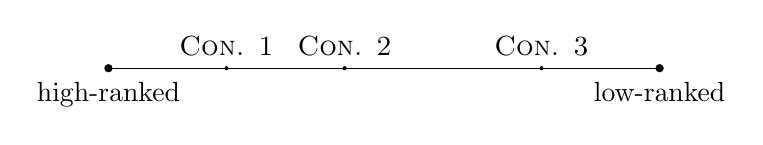
\begin{tikzpicture}
  \draw [circle, inner sep=0pt, minimum size=1.5pt] (0,0) -- +(7,0) ;
  \node[fill, label=below:{high-ranked}, circle, inner sep=0pt, minimum size=3.0pt] (d) at (0,0) {};  
  \node[fill, label=below:{low-ranked}, circle, inner sep=0pt, minimum size=3.0pt] (e) at (7,0) {};    
  \node[fill, label=above:\textsc{Con. 1}, circle, inner sep=0pt, minimum size=1.5pt] (a) at (1.5,0) {};
  \node[fill, label=above:\textsc{Con. 2}, circle, inner sep=0pt, minimum size=1.5pt] (b) at (3.0,0) {};  
  \node[fill, label=above:\textsc{Con. 3}, circle, inner sep=0pt, minimum size=1.5pt] (c) at (5.5,0) {};  
\end{tikzpicture}
\end{figure}

Now, the model has to implement a way to deal with gradient grammaticality, solving the many issues Standard Optimality Theory has with modeling the implicit object construction (debated  \vrefpage{ot_bad_dobjdrop}). Stochastic Optimality Theory achieves this result by means of the Gradual Learning Algorithm, which is intended to be an improvement on the Constraint Demotion algorithm \parencite{TesarSmolensky1993learnability} used in Standard Optimality Theory. Using the Gradual Learning Algorithm to build a Stochastic Optimality Theoretic grammar is a sensible choice for linguists dealing with any phenomenon where a given input generates candidates with no unique winner, such as language change (with different winners at different times in history), language development (with different winners at different times in the child's life), and complex synchronic phenomena such as the indefinite object drop (with different winners at the same time, based on the way constraint interact).\\
Stochastic Optimality Theory allows more than one candidate to be optimal at the same time by allowing constraints to "float" on the continuous scale, as if perturbed by numerical noise at the moment of evaluation. In practice, this is possible by assigning to each constraint a full range of values, centered on what was previously a single point on the scale (now called "ranking value"). Given the range of values, the specific value used at evaluation time is called an "evaluation point". Most importantly, the constraint ranking ranges are defined as probability distributions, and distribution overlap determines the probability of two constraint re-ranking with respect to one another. As illustrated in \reffig{stochot_gaussians1} and \reffig{stochot_gaussians2}, probability distributions in Stochastic Optimality Theory are \textit{normal} distributions. The Gaussian curves are defined by their mean value, which is the ranking value, and their standard deviation, which determines how broad the curve is.\sidenote{Let $\mu$ be the mean value of the distribution and $\sigma$ the standard deviation. The normal distribution is a function defined by the equation:
$$ f(x) = \frac{1}{\sigma\sqrt{2\pi}}e^{-\frac{1}{2}(\frac{x-\mu}{\sigma})^2} $$
} Since all constraints are assigned the same normal distribution in traditional Stochastic Optimality Theory, the actual value of the standard deviation (the "evaluation noise") has no effect on the constraint re-ranking, and it is arbitrarily set at 2 (a different approach to this matter is provided in \textcite{reynolds1994variation, nagy1997optimality}). At evaluation time the selection point will occur most probably in correspondence of the ranking value (given the properties of normal distributions), and its probability steady declines as its value departs from the center of the distribution (i.e. the ranking value).\\
Going back to the simple state of affairs illustrated in \reffig{stot_contranking}, it is evident from \reffig{stochot_gaussians1} that the floating-constraint model makes it now possible for \textsc{Constraint 1} and \textsc{Constraint 2} to re-rank. In the picture, \textsc{Constraint 1} has a ranking value of 6.5 and \textsc{Constraint 2} a ranking value of 4, ordered from the higher-ranked to the lower-ranked as in the custom of Optimality Theory. In particular, as shown by the overlapping curves, the two constraints re-rank freely when the selection points are comprised between 4 and 6.5, and it is much more probable for \textsc{Constraint 1} to outrank \textsc{Constraint 2} than the opposite (graphically, there is only a small area where the curve for \textsc{Constraint 2} is above the curve for \textsc{Constraint 1}, for x values between 4 and 5.25).

\pgfmathdeclarefunction{gauss}{2}{%
  \pgfmathparse{1/(#2*sqrt(2*pi))*exp(-((x-#1)^2)/(2*#2^2))}%
}

\begin{figure}[htb]
\caption{Constraint re-ranking distribution in Stochastic Optimality Theory (overlapping constraints).}
\labfig{stochot_gaussians1}
\begin{tikzpicture}
\begin{axis}[
  no markers, domain=0:10, samples=100, xscale=-1,
  axis lines*=left, xlabel=$x$, ylabel=$y$, 
  every axis y label/.style={at=(current axis.above origin),anchor=south},
  every axis x label/.style={at=(current axis.left of origin),anchor=east},
  height=3cm, width=10cm, % height=5cm, width=12cm,
  xtick={4,6.5}, ytick=\empty,
  enlargelimits=false, clip=false, axis on top,
  grid = major
  ]
  \addplot [fill=cyan!20, draw=none, domain=0:6.5] {gauss(6.5,1)}
  \closedcycle;
  \addplot [fill=cyan!20, draw=none, domain=4:6.5] {gauss(4,1)}
  \closedcycle;
  \addplot [very thick,dotted,cyan!50!black] {gauss(4,1)};
  \addplot [very thick,cyan!50!black] {gauss(6.5,1)};
% \draw [yshift=-1.2cm, latex-latex](axis cs:4,0) -- node [fill=white] {$1.96\sigma$} (axis cs:5.96,0);
\draw [yshift=-0.5cm, latex-latex](axis cs:4,0) -- node [fill=white] {\textsc{Constr. 2}} (axis cs:4,0);
\draw [yshift=-0.5cm, latex-latex](axis cs:6.5,0) -- node [fill=white] {\textsc{Constr. 1}} (axis cs:6.5,0);
\end{axis}
\end{tikzpicture}
\end{figure}

Instead, \textsc{Constraint 2} and \textsc{Constraint 3} never re-rank, since their probability distributions in \reffig{stochot_gaussians2} never overlap (ranking values have been randomly assigned in the picture just for the argument's sake). In situations such as this, the constraint ranking on a continuous scale just reproduces the results of the categorical ranking yielded in standard Optimality Theory, i.e. strict domination.

\begin{figure}[htb]
\caption{Constraint re-ranking distribution in Stochastic Optimality Theory (non-overlapping constraints).}
\labfig{stochot_gaussians2}
\begin{tikzpicture}
\begin{axis}[
  no markers, domain=0:10, samples=100, xscale=-1,
  axis lines*=left, xlabel=$x$, ylabel=$y$,
  every axis y label/.style={at=(current axis.above origin),anchor=south},
  every axis x label/.style={at=(current axis.left of origin),anchor=east},
  height=3cm, width=10cm, % height=5cm, width=12cm,
  xtick={2,8}, ytick=\empty,
  enlargelimits=false, clip=false, axis on top,
  grid = major
  ]
%   \addplot [fill=cyan!20, draw=none, domain=0:5.96] {gauss(8,1)} \closedcycle;
  \addplot [very thick,dotted,cyan!50!black] {gauss(2,1)};
  \addplot [very thick,cyan!50!black] {gauss(8,1)};
% \draw [yshift=-1.2cm, latex-latex](axis cs:2,0) -- node [fill=white] {$1.96\sigma$} (axis cs:5.96,0);
\draw [yshift=-0.5cm, latex-latex](axis cs:2,0) -- node [fill=white] {\textsc{Constr. 3}} (axis cs:2,0);
\draw [yshift=-0.5cm, latex-latex](axis cs:8,0) -- node [fill=white] {\textsc{Constr. 2}} (axis cs:8,0);
\end{axis}
\end{tikzpicture}
\end{figure}

The Gradual Learning Algorithm uses these premises to assign an empirically motivated ranking value to each constraint, modulating its outcome based on an error-driven procedure. The full details of how the algorithm works, which the reader will find in \textcite{BoersmaHayes2001empirical} are outside the scope of this chapter. For the purposes of my dissertation, it is important to note that Stochastic Optimality Theory provides an optimal environment to create a model of object drop. Let us consider a simple example such as \ref{mock_simple_dobj}, where the verb \textit{to eat} is used transitively in \ref{mock_simple_dobj1} and intransitively in \ref{mock_simple_dobj2}, and let us ignore the effect of the many factors influencing object drop (discussed in \refch{factors}) for the time being. Both \ref{mock_simple_dobj1} and \ref{mock_simple_dobj2} are grammatical, but the latter is judged slightly less acceptable than the former on average by some hypothetical native speakers.
% \vspace{-0.5cm} % PER AGGIUSTARE LO SPAZIO PRIMA DEGLI ESEMPI!
\ex. \label{mock_simple_dobj} \a. \label{mock_simple_dobj1} John is eating pizza. \hfill 7
\b. \label{mock_simple_dobj2} John is eating. \hfill 6.5

In our factor-agnostic model of object drop, we would posit just two conflicting constraints in the spirit of Optimality Theory (\refsec{classicot}): \textsc{*Internal Argument Structure}, a markedness constraint penalizing the presence of an overt direct object in the output, and \textsc{Faithfulness to Argument Structure}, a faithfulness constraint requiring all the arguments in the input to be also realized in the output. In a standard Optimality Theoretic analysis of the candidate set in \ref{mock_simple_dobj}, \textsc{Faithfulness to Argument Structure} would be ranked above \textsc{*Internal Argument Structure} and make \ref{mock_simple_dobj1} the only winner in the competition, with no reference to the slight acceptability difference. A Stochastic Optimality Theoretic model would solve the problem, so that \textsc{Faithfulness to Argument Structure} would indeed be ranked above \textsc{*Internal Argument Structure} most of the times, but with a large overlap between the two probability distributions (see \reffig{stochot_gaussians_dobj}). Crucially, one constraint outranks the other only probabilistically, while in the standard Optimality Theoretic model it would do so in an absolute sense due to strict domination.

\begin{figure}[htb]
\caption{Constraint re-ranking distribution in Stochastic Optimality Theory relative to Example \ref{mock_simple_dobj}.}
\labfig{stochot_gaussians_dobj}
\begin{tikzpicture}
\begin{axis}[
  no markers, domain=0:10, samples=100, xscale=-1,
  axis lines*=left, xlabel=$x$, ylabel=$y$, 
  every axis y label/.style={at=(current axis.above origin),anchor=south},
  every axis x label/.style={at=(current axis.left of origin),anchor=east},
  height=3cm, width=8cm, % height=5cm, width=12cm,
  xtick={5.5,6.5}, ytick=\empty, xticklabels={,,},
  enlargelimits=false, clip=false, axis on top,
  grid = major
  ]
%   \addplot [fill=cyan!20, draw=none, domain=0:6.5] {gauss(6.5,1)}
%   \closedcycle;
%   \addplot [fill=cyan!20, draw=none, domain=5.5:6.5] {gauss(5.5,1)}
%   \closedcycle;
  \addplot [very thick,dotted,cyan!50!black] {gauss(5.5,1)};
  \addplot [very thick,cyan!50!black] {gauss(6.5,1)};
% \draw [yshift=-1.2cm, latex-latex](axis cs:4,0) -- node [fill=white] {$1.96\sigma$} (axis cs:5.96,0);
\draw [yshift=2.0cm, latex-latex](axis cs:5.5,0) -- node [fill=white] {\textsc{*Int Arg}} (axis cs:5.5,0);
\draw [yshift=-0.5cm, latex-latex](axis cs:6.5,0) -- node [fill=white] {\textsc{Faith Arg}} (axis cs:6.5,0);
\end{axis}
\end{tikzpicture}
\end{figure}

The use of Stochastic Optimality Theory to define a working model of the implicit object construction, aware of the effect of several predictors (\refch{factors}) and the fact that different transitive verbs are differently prone to be used intransitively, is the topic of the next section.

\section{Medina's (2007) model} \labsec{medinamodel}

\textcite{Medina2007} created a Stochastic Optimality Theoretic model of the indefinite object drop. An implicit object output, generated by Gen on the basis of the input (\refsec{inputmedina}), is evaluated against a set of conflicting constraints (\refsec{constraintsmedina}). The constraints stem directly from the set of object drop predictors chosen by the author (\refsec{predictorsmedina}), and get re-ranked with respect to the verb's semantic selectivity (\refsec{rankingmedina}), computed as the Selectional Preference Strength by \textcite{Resnik1993, Resnik1996}. The way this model implements a probabilistic ranking of the constraints ensures not only that both implicit and overt objects are allowed in the grammar, but also that an implicit object output has a relative gradient grammaticality across different verbs.


\subsection{The input and the output} \labsec{inputmedina}

As I mentioned in \refsec{classicot}, Optimality Theory requires the input to syntactic optimization to contain the relevant lexical and semantic components that will be mapped to the syntactically well-formed output forms. Since \textcite{Medina2007} defines a model of the indefinite object drop, her input has to provide all the information necessary to generate the two outputs in  \ref{medina_output_generic}:
% \vspace{-0.5cm} % PER AGGIUSTARE LO SPAZIO PRIMA DEGLI ESEMPI!
\ex. \label{medina_output_generic} \a. John was writing.
\b. John was writing something.

Hence, at the very least the input contains a transitive verb with its complete predicate-argument structure, i.e. a specified subject and an unspecified object. Since the model does not deal with \textit{specified} object drop, the input to the model cannot generate an output with a specific overt object as in \ref{medina_output_wrong}. To put it better, \textcite[70-71]{Medina2007} observes that this output may actually be in the candidate set, but it is always ruled out by a high-ranking faithfulness constraint that keeps output candidates from containing semantically richer information than in the input.
% \vspace{-0.5cm} % PER AGGIUSTARE LO SPAZIO PRIMA DEGLI ESEMPI!
\ex. \label{medina_output_wrong} John was writing a book.

In addition to this, the input will also feature all the relevant predictors of object drop used by the author, i.e. semantic selectivity (operationalized as Resnik's Selectional Preference Strength), telicity, and perfectivity. Thus, inputs in \textcite{Medina2007} have the form \ref{medina_input_generic}:
% \vspace{-0.5cm} % PER AGGIUSTARE LO SPAZIO PRIMA DEGLI ESEMPI!
\ex. \label{medina_input_generic} verb (x,y), x = subject, y = unspecified, SPS = \textit{numerical value}, [+ Past], [$\pm$ Telic], [$\pm$ Perfective]

The tense feature is fixed at [+ Past] since the author only modeled past tenses for consistency, but there is no hard theoretical constraint on this. In theory, it would indeed be possible to create similar inputs with other tenses. Looking at a specific case, the input generating the outputs in \ref{medina_output_generic} would look like \ref{medina_input_teach}.
% \vspace{-0.5cm} % PER AGGIUSTARE LO SPAZIO PRIMA DEGLI ESEMPI!
\ex. \label{medina_input_teach} write (x,y), x = John, y = unspecified, SPS = 2.54\sidenote{This is the value of Selectional Preference Strength that Resnik obtained by performing the computation over the Brown corpus of English \parencite[150]{Resnik1996}, also reported in \textcite[114]{Medina2007}}, [+ Past], [-Telic], [- Perfective]

Let us take a closer look at how the three predictors chosen by Medina are implemented in her model.

%  È GIUSTO CHE QUI GLI OGGETTI SIANO INDEFINITI!!! NELL'ESPERIMENTO SONO OVERT PERCHÈ NON RIENTRANO NEL MODELLO OT!!! 83 pdf Medina

\subsection{Predictors} \labsec{predictorsmedina}

\paragraph{Semantic selectivity} \textcite{Medina2007} uses semantic selectivity as a proxy to gauge the recoverability of a transitive verb's direct objects, which the reader will remember being a major determiner of object drop based on the information discussed in \refsec{recoverability}. As a quick recap, I will just note that the recoverability of the broad class of a direct object of a verb correlates with the grammaticality of sentences featuring that same verb used intransitively, as in \ref{recap_sps}.
% \vspace{-0.5cm} % PER AGGIUSTARE LO SPAZIO PRIMA DEGLI ESEMPI!
\ex. \label{recap_sps} \a. John ate $\varnothing$\textsubscript{dObj}. \\ $\longrightarrow$ The omitted object belongs to the category of Edibles.
\b. *John made $\varnothing$\textsubscript{dObj}. \\ $\longrightarrow$ The omitted object can be virtually anything.

In theory, it would be possible to treat the semantic selectivity of a transitive verb with respect to its direct objects as a binary feature and be done with it. However, this choice would be quite poor both from a methodological point of view, since there is no clear-cut criterion to tell apart recoverable-object and non-recoverable-object verbs, and from a usability point of view, since binary selectivity would be scarcely informative with respect to object drop.\\
Making use of the experimental literature on the matter, \textcite{Medina2007} decided to operationalize semantic selectivity using the Selectional Preference Strength measure developed by \textcite{Resnik1993, Resnik1996}. Resnik quantifies the selectional preferences of transitive verbs in an information-theoretical model which encodes semantic selectivity as the relative entropy between the distribution of WordNet \parencite{beckwith1991wordnet, Miller1995} classes for all the direct objects in a corpus and the distribution of WordNet classes for the direct objects of a specific verb. I will discuss the mathematical meaning and the computational details of Resnik's Selectional Preference Strength in \refsec{predictor_sps}, where I will also present an update of his measure I contributed to create \parencite{CappelliLenciPISA}, powered by distributional semantics and word embeddings.\\
Here, I will only point out how suitable Resnik's measure is for the purposes of Medina's model of object drop. First of all, the Selectional Preference Strength takes a numerical value (a non-null positive real number) on a continuous scale, which it makes it perfect to capture the fact that semantic selectivity is not a binary variable. In particular, the narrower the selectional preferences of a verb are (i.e. the more recoverable its direct objects are), the greater the Selectional Preference Strength of that verb is. Most conveniently for Medina's thesis in acquisitional linguistics, whose scope goes far beyond the coding of computational technicalities, \textcite[150]{Resnik1996} provides the Selectional Preference Strength scores computed for 34 English verbs over the Brown corpus \parencite{kucera1967brownCorpus}, the CHILDES corpus \parencite{macwhinney2000childesCorpus}, and human subject norms. While being a modest set of data, this collection of scores has all the data Medina needed to build her model of the implicit object construction, and to this day it is still a valuable resource for anyone looking into models of semantic selectivity.


\paragraph{Telicity} Telicity has been proven to be an important predictor of the omissibility of direct objects in \refsec{telicity}. Medina encodes it as a binary variable, so that the transitive verbs she tested (Resnik's 34 ones) are tagged as either telic or atelic. Doing so, however, is less straightforward than it may seem at a first glance.\\
Telicity, in its typical interpretation, is a property of predicates \parencite{Vendler1957, dowty2012word1979}. This means that the (a)telicity feature may only be assigned to complete verb phrases, complete with arguments and adjuncts, and not to bare verb heads (see the simplified tree in \reffig{telicity_at_vp_tree}). Under this view, predicates are telic if the event they describe have an endpoint (encoded as a direct object), or they are atelic if they don't. As a logical consequence, the same verb would be considered telic when used transitively and atelic when used intransitively \parencite{OlsenResnik1997, Mittwoch1982}.

\begin{figure}[htb]
\caption{Simplified syntax tree illustrating the traditional interpretation of telicity as a property of predicates, not verb heads.}
\labfig{telicity_at_vp_tree}
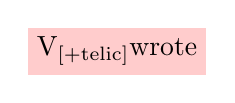
\begin{tikzpicture}
\Tree [.TP [.DP \edge[roof]; {John} ] [.T' [. \node(x){T\\$\varnothing$\textsubscript{[+past]}}; ] [.\node[fill=green!20] {VP\textsubscript{[+telic]} };[.V' [.\node[fill=red!20] {V\textsubscript{\sout{[+telic]}}\\wrote}; ] [.DP \edge[roof]; {a book} ] ] ] ] ]
% \draw[semithick, <-] (x) to [bend right=70] (y);
\end{tikzpicture}
\end{figure}

As Medina points out, the telicity taking scope over a whole verb phrase poses a severe problem with respect to the use of telicity as a predictor of object drop. How can an object-dropping transitive verb be always considered (a)telic, if the very act of adding or dropping its object alters its telicity? Medina's solution to this conundrum makes use of the analysis of telicity as a privative feature by \textcite{Olsen1997telicity-privative}. Let us discuss this approach in more detail.\\
According to \textcite[32]{Olsen1997telicity-privative}, telicity is a semantic feature verbs have if the event they denote can have an endpoint or a result, regardless of whether they actually attain it or not. Based on this, [+telic] verbs cannot lose the feature even if the endpoint is not realized as a syntactic constituent. On the contrary, atelicity is a cancelable conversational implicature, so [-telic] verbs can be interpreted as either having or not having an inherent endpoint or result. Olsen (followed by Medina) actually uses the notation [0 Telic] to indicate the feature of verbs which lack telic denotation, but in this thesis I will use a more transparent opposition between [+telic] and [-telic] verbs. Now informed about the underlying theory, the reader will be able to interpret the [-telic] feature as Olsen intended.\\
By virtue of this particular interpretation of telicity, Medina considers [+telic] verbs such as \textit{to make} and [-telic] verbs such as \textit{to eat}. Telicity (or lack thereof) is assigned to each verb on the basis of three tests\sidenote{All the examples in the list are taken \textit{verbatim} from \textcite[302-303]{Medina2007}.}.

\begin{itemize}
    \item \textbf{The \textit{in/for} test} \parencite{dowty2012word1979, Vendler1957}. Predicates featuring [+telic] verbs \ref{telicitytest_infor1} allow more easily \textit{in-X-time} temporal adverbs and less easily \textit{for-X-time} temporal adverbs, while predicates with [-telic] verbs \ref{telicitytest_infor2} have the reverse preference pattern.
    
\ex. \label{telicitytest_infor} \a. \label{telicitytest_infor1} Michelle made some stuff in/*for five minutes.
\b. \label{telicitytest_infor2}  Michelle read *in/for five minutes.
    
    \item \textbf{The \textit{almost} test} \parencite{dowty2012word1979}. The adverb \textit{almost} allows [+telic] verbs \ref{telicitytest_almost1} to have two interpretations (the event has begun but hasn't finished yet; the event hasn't begun yet), while [-telic] verbs \ref{telicitytest_almost2} can have only one (the event hasn't begun yet).
    
\ex. \label{telicitytest_almost} \a. \label{telicitytest_almost1} Tony almost packed.\\ $\longrightarrow$  Tony started packing, but hasn’t finished yet. \\ $\longrightarrow$  Tony was about to pack but hadn’t yet started.
\b. \label{telicitytest_almost2} Tony almost ate.\\ $\longrightarrow$  \sout{Tony started eating, but hasn’t finished yet.} \\ $\longrightarrow$  Tony was about to eat but hadn’t yet started.
    
    \item \textbf{The \textit{counting} test} \parencite{bach1986algebra}. It is more acceptable to count [+telic] predicates \ref{telicitytest_counting1} than [-telic] ones \ref{telicitytest_counting2}, or in other words, counted [+telic] predicates are interpreted as a single event with repeated acts, while counted [-telic] predicates are interpreted as repeated, distinct events. This is the most controversial test out of the three Medina chose to use.

\ex. \label{telicitytest_counting} \a. \label{telicitytest_counting1} Edgar opened some stuff three times.
\b. \label{telicitytest_counting2}  Edgar watched three times.

\end{itemize}

Verbs are tested in combination with an implicit object or in an intransitive sentence. A transitive verb tested this way is [+telic] if at least two tests out of three yield a telic interpretation or [-telic] otherwise, based on the assumption that the verb lacks telic denotation (i.e. is atelic) if it can elicit both a telic and an atelic interpretation. As I will discuss in more detail in \refsec{predictor_telicity}, while the \textit{in/for} test is a largely reliable diagnostic for telicity, the other two tests are somewhat problematic.


\paragraph{Perfectivity} While telicity (i.e. lexical aspect) is a semantic property of individual verbs, as illustrated in the previous paragraph, perfectivity (i.e. grammatical aspect) in English is morphologically marked. As noted in \refsec{inputmedina}, \textcite{Medina2007} only modeled inputs in the past tense. With respect to the morphological markers of (im)perfectivity, the author followed \textcite{Olsen1997telicity-privative} in realizing [+perfective] inputs with perfect morphology, in the form "\textit{have} + past participle of the verb" \ref{medina_perfectivity1}, and [-perfective] inputs with progressive morphology, in the form "\textit{be} + verb + \textit{-ing}" \ref{medina_perfectivity2}.

\ex. \label{medina_perfectivity} \a. \label{medina_perfectivity1} John had written a book.
\b. \label{medina_perfectivity2}  John was writing a book.

In my own model of object drop, I mark (im)perfective aspect on English verbs using the same morphology as in \textcite{Medina2007}, and I device a similar strategy for my Italian stimuli (\refsec{predictor_perfectivity}).


\subsection{Constraints and constraint ranking} \labsec{constraintsmedina}

For each input to the optimization in Medina's model, the two outputs (one with an overt object, one with an implicit object, as detailed in \refsec{inputmedina}) are evaluated against the four constraints in \ref{medina_constraints}. Their label and definition are taken directly from \textcite[72]{Medina2007}.

% A set of four candidates is being evaluated against the same one markedness and three faithfulness constraints

\ex. \label{medina_constraints} 
\a. \label{medina_constraints_intarg} \textsc{*Int Arg (*Internal Argument Structure)}\\ The output must not contain an overt internal argument (that is to say, a direct object).
\b. \label{medina_constraints_faith} \textsc{Faith Arg (Faithfulness to Argument Structure)}\\ All arguments in the input must be present in the output.
\c. \label{medina_constraints_telic} \textsc{Telic End (Telic Endpoint)}\\ The endpoint of a [+ Telic] event must be bounded by the presence of an overt argument in the output.
\c. \label{medina_constraints_perf} \textsc{Perf Coda (Perfective Coda)}\\ The coda of a perfective event [+ Perfective] must be identified by the presence of an overt argument in the output.

Let us discuss each constraint more extensively. \textsc{*Int Arg} \ref{medina_constraints_intarg} is a markedness constraint belonging to a broader class of economy-of-structure constraints, \textsc{*Struc} \parencite{buchwald2002recoverability, hartkemeyer2000ot}, operating in syntax and every other domain of grammar. By penalizing candidates with an overt object, which have a greater degree of syntactic structure than candidates with an implicit object, \textsc{*Int Arg} is the only constraint in Medina's set to favor implicit-object candidates. As I will explain in \refsec{rankingmedina}, this unique behavior of \textsc{*Int Arg} is not just intended, but downright necessary for the probabilistic re-ranking of the constraint to happen.\\
\textsc{Faith Arg} is a faithfulness constraint requiring that all arguments in the input be overtly realized in the output, thus penalizing candidates with an implicit object. As discussed in \refsec{classicot}, faithfulness constraints are a unique feature of Optimality Theory, created in order to conflict with economy-of-structure markedness constraints like the framework requires. Without faithfulness constraints, the optimal candidate would always be the least marked one, i.e. the one to violate the lowest-ranked constraints \parencite[3]{legendre2001introduction}. In the specific case of Medina's model, \textsc{Faith Arg} conflicts directly with \textsc{*Int Arg}, determining a state of affairs that closely resembles the situation previously described in \reffig{stochot_gaussians_dobj}. The picture is made more complex by the interaction of two additional constraints and the inclusion of semantic selectivity in the model.\\
Finally, the markedness constraints \textsc{Telic End} and \textsc{Perf Coda} are the Optimality Theoretic implementations of telicity (\refsec{telicity}) and perfectivity (\refsec{perfectivity}) as predictors of object drop, both penalizing object-dropping output candidates. Notably, while \textsc{*Int Arg} and \textsc{Faith Arg} are always active regardless of the input features, \textsc{Telic End} and \textsc{Perf Coda} are only actively used by the \textsc{Eval} component if the input is, respectively, [+telic] and [+perfective]. Let us consider the examples in \reftab{medina2007_Ytel_Yperf} to \reftab{medina2007_Ntel_Nperf}, adapted from \textcite{Medina2007}. The absence of the pointing hand indicates that no winner has been chosen among the candidates, since these examples are just here to illustrate the possible violation profiles determined by different inputs. In the same spirit, the dotted lines show that no constraint ranking (neither in standard nor in stochastic Optimality Theory) has been determined.\\
A transitive verb which is both telic and perfective, such as \textit{to catch} in \reftab{medina2007_Ytel_Yperf}, has a full constraint violation profile involving all the four constraints at play in Medina's model. Instead, the output candidates for a telic but imperfective input verb (as \textit{to catch} in \reftab{medina2007_Ytel_Nperf}) only violate \textsc{*Int Arg}, \textsc{Faith Arg}, and \textsc{Telic End}. In this situation, \textsc{Perf Coda} is vacuously satisfied, i.e. there is no candidate in the candidate set with the ability to violate the constraint (given that it is violated by object-dropping perfective candidates, and here there is none). Similarly, \textsc{Telic End} is vacuously satisfied in \reftab{medina2007_Ntel_Yperf}, and both \textsc{Telic End} and \textsc{Perf Coda} are vacuously satisfied in \reftab{medina2007_Ntel_Nperf}.

\begin{table}[htb] % the "htb" makes table env unfloaty
\caption{Optimality Theory tableau illustrating the constraint violation profile in the model of object drop by \textcite{Medina2007}, relative to a telic perfective verb.}
\labtab{medina2007_Ytel_Yperf} % \hand a.
\begin{adjustbox}{max width=\textwidth}
\begin{tabular}{|ll||c;{1pt/1pt}c;{1pt/1pt}c;{1pt/1pt}c|}\hline   
      & \vtop{\hbox{\strut catch (x,y), x = Jack, y = unspecified, SPS = n/a, }\hbox{\strut [+Past], [+Telic], [+Perfective]}}  & \textsc{\rotatebox[origin=c]{90}{ *Int Arg }}  &  \textsc{\rotatebox[origin=c]{90}{ Faith Arg }} & \textsc{\rotatebox[origin=c]{90}{ Telic End }} &
      \textsc{\rotatebox[origin=c]{90}{ Perf Coda }}\\
      \hline\hline
a. & Jack had caught.     &   &  *   & * & *\\ \hline
b. & Jack had caught something.     & *  &   &  & \\ \hline
\end{tabular}
\end{adjustbox}
\end{table}

\begin{table}[htb] % the "htb" makes table env unfloaty
\caption{Optimality Theory tableau illustrating the constraint violation profile in the model of object drop by \textcite{Medina2007}, relative to a telic imperfective verb.}
\labtab{medina2007_Ytel_Nperf} % \hand a.
\begin{adjustbox}{max width=\textwidth}
\begin{tabular}{|ll||c;{1pt/1pt}c;{1pt/1pt}c;{1pt/1pt}c|}\hline   
      & \vtop{\hbox{\strut catch (x,y), x = Jack, y = unspecified, SPS = n/a, }\hbox{\strut [+Past], [+Telic], [-Perfective]}}  & \textsc{\rotatebox[origin=c]{90}{ *Int Arg }}  &  \textsc{\rotatebox[origin=c]{90}{ Faith Arg }} & \textsc{\rotatebox[origin=c]{90}{ Telic End }} &
      \textsc{\rotatebox[origin=c]{90}{ \textcolor{gray}{Perf Coda} }}\\
      \hline\hline
a. & Jack was catching.     &   &  *   & * & \\ \hline
b. & Jack was catching something.     & *  &   &  & \\ \hline
\end{tabular}
\end{adjustbox}
\end{table}

\begin{table}[htb] % the "htb" makes table env unfloaty
\caption{Optimality Theory tableau illustrating the constraint violation profile in the model of object drop by \textcite{Medina2007}, relative to an atelic perfective verb.}
\labtab{medina2007_Ntel_Yperf} % \hand a.
\begin{adjustbox}{max width=\textwidth}
\begin{tabular}{|ll||c;{1pt/1pt}c;{1pt/1pt}c;{1pt/1pt}c|}\hline   
      & \vtop{\hbox{\strut eat (x,y), x = Jack, y = unspecified, SPS = n/a, }\hbox{\strut [+Past], [-Telic], [+Perfective]}}  & \textsc{\rotatebox[origin=c]{90}{ *Int Arg }}  &  \textsc{\rotatebox[origin=c]{90}{ Faith Arg }} & \textsc{\rotatebox[origin=c]{90}{ \textcolor{gray}{Telic End} }} &
      \textsc{\rotatebox[origin=c]{90}{ Perf Coda }}\\
      \hline\hline
a. & Jack had eaten.     &   &  *   &  & *\\ \hline
b. & Jack had eaten something.     & *  &   &  & \\ \hline
\end{tabular}
\end{adjustbox}
\end{table}

\begin{table}[htb] % the "htb" makes table env unfloaty
\caption{Optimality Theory tableau illustrating the constraint violation profile in the model of object drop by \textcite{Medina2007}, relative to an atelic imperfective verb.}
\labtab{medina2007_Ntel_Nperf} % \hand a.
\begin{adjustbox}{max width=\textwidth}
\begin{tabular}{|ll||c;{1pt/1pt}c;{1pt/1pt}c;{1pt/1pt}c|}\hline   
      & \vtop{\hbox{\strut eat (x,y), x = Jack, y = unspecified, SPS = n/a, }\hbox{\strut [+Past], [-Telic], [-Perfective]}}  & \textsc{\rotatebox[origin=c]{90}{ *Int Arg }}  &  \textsc{\rotatebox[origin=c]{90}{ Faith Arg }} & \textsc{\rotatebox[origin=c]{90}{ \textcolor{gray}{Telic End} }} &
      \textsc{\rotatebox[origin=c]{90}{ \textcolor{gray}{Perf Coda} }}\\
      \hline\hline
a. & Jack was eating.     &   &  *   &  & \\ \hline
b. & Jack was eating something.     & *  &   &  & \\ \hline
\end{tabular}
\end{adjustbox}
\end{table}

So far, so good. However, the attentive reader will have noticed that no mention has been made of semantic selectivity among the constraints at play, even though it has been said to be a crucial predictor of object drop (\refsec{recoverability}, \refsec{predictorsmedina}). As \textcite[76]{Medina2007} observes, it would indeed be easy to define an \textsc{*Overt Recoverable Object} constraint penalizing overt objects occurring with high-selectivity verbs, or a \textsc{*Non-recoverable Implicit Object} constraint penalizing implicit objects occurring with low-selectivity verbs. This works perfectly for binary predictors such as telicity and perfectivity, but semantic selectivity is not a binary predictor (as noted at the beginning of \refsec{predictorsmedina}). Not only is it quantified by means of a continuous numerical variable, but it is structurally impossible to define a threshold value separating high- and low-selectivity transitive verbs. In the original works about a computational model of semantic selectivity as a proxy to argument recoverability \parencite{Resnik1993, Resnik1996}, the author himself observed that albeit his Selectional Preference Strength measure correlates well with the acceptability of implicit objects, there are indeed some cases where a high-SPS verb does not allow for its object to be dropped (e.g. \textit{to hang, to wear}). For this reason, as I will detail further in the next section, SPS will play a crucial role in Medina's probabilistic constraint ranking, despite not being defined as a constraint \textit{per se}.\\
The gradient nature of object recoverability, be it computed via SPS \parencite{Resnik1993, Resnik1996} or PISA \parencite{CappelliLenciPISA}, makes it a bad candidate for constraint-hood. Moreover, even if it were possible to binarize it into a viable constraint, it would still suffer from a problem afflicting all the binary constraints at play, i.e. out-of-range output generation both within-constraint and across constraints. In other words, each constraint in the model under- or over-generates outputs across verbs, since experimental data show that some telic verbs occur with implicit objects while others don't, that perfective aspect favors implicit objects but doesn't force them, and so on. This is normal, expected behavior for classic OT constraints, easily solved by means of re-ranking in order to select the winner candidate. However, in this case the state of affairs is more complicated.\\
As shown in \reftab{medina2007_Ytel_Yperf} to \reftab{medina2007_Ntel_Nperf}, forcing the implicit object construction into a standard Optimality Theoretic model has two major drawbacks. One is that the same constraint violations apply to any verb with a given aspectual profile, meaning that a tableau like \reftab{medina2007_Ntel_Yperf} would apply to \textit{to eat} and to any other atelic perfective input (since in standard Optimality Theory, the ranking order of the constraint has to be consistent within the same language). As observed right before in this paragraph, this does not match the actual linguistic data on object drop. The second issue with such a model is that it only allows for a single winner out of a candidate set, so that (also considering the previous problem) for a given aspectual profile, regardless of the specific verb in the input, the direct object would be either obligatory, or obligatorily dropped. Looking again at tableaux \reftab{medina2007_Ytel_Yperf} to \reftab{medina2007_Ntel_Nperf}, the model would determine which of the two candidates would win the competition solely based on the relative ranking of \textsc{*Int Arg} with respect to any of the other constraints (since the relative ranking of \textsc{Faith Arg}, \textsc{Telic End}, and \textsc{Perf Coda} is irrelevant for the purposes of electing a winner). Given that the implicit object construction is felicitous depending on the interaction of several factors, and given that no factor or combination of factors actively forces or prohibits object drop, the logical conclusion is that a standard Optimality Theoretic model of object drop is lacking.\\
Taking all of this into consideration, a non-standard Optimality Theoretic comprehensive model of the implicit object construction based on the linguistic factors hereby described has to account for two aspects, i.e.
\begin{enumerate}
    \item incorporating semantic selectivity (a continuous, non-binary factor) into the model, and
    \item having the model yield outputs with varying degrees of grammaticality, instead of having a winner and a loser.
\end{enumerate}

\subsection{Defining a probabilistic constraint ranking} \labsec{rankingmedina}
\paragraph{Introduction} \textcite{Medina2007} built such a model under the premises of Stochastic Optimality Theory, whose tenets I introduced in \refsec{stochot}. This framework accounts for gradient grammaticality out-of-the-box, since it assigns each candidate a probability of it being the winner, to be interpreted as a degree of acceptability. As for the implementation of semantic selectivity as a continuous factor, Medina came up with a personal variation on Stochastic Optimality Theory.\\
As noted before in tableaux \reftab{medina2007_Ytel_Yperf} to \reftab{medina2007_Ntel_Nperf}, the winner in a Standard Optimality Theoretic model is determined based on the ranking of \textsc{*Int Arg} relative to the other three constraints at play. The same would hold true for a traditional Stochastic Optimality Theoretic version of the same model, where all constraints would be assigned a given normal distribution with a fixed evaluation noise (fully described by its standard deviation). Medina's stochastic model obtains the probability of \textsc{*Int Arg} dominating the other three constraints as a function of the verb's semantic selectivity, computed using Resnik's Selectional Preference Strength \parencite{Resnik1993,Resnik1996}. Compared with traditional Stochastic Optimality Theory, Medina's proposal achieves the same goal of having candidates with \textit{gradient} grammaticality (instead of a single absolute winner), while having two advantages:
\begin{itemize}
    \item implementing semantic selectivity in the model properly, and
    \item defining the relative ranking of \textsc{*Int Arg} with respect to the other three constraints as independent computations, yielding fine-grained interactions of semantic selectivity with telicity, perfectivity and faithfulness to the input.
\end{itemize}
In such a model, the grammaticality of candidates is assessed across all possible constraint re-rankings, each of which is assigned a probability by the model. Medina's implementation of this model stems from a three-step logic:
\begin{enumerate}
    \item the probability of \textsc{*Int Arg} dominating each of the other constraints is expressed as a function of the input verb's semantic selectivity, computed via Resnik's Selectional Preference Strength
    \item the values of the function are used to compute the relative probabilities of each of the four possible re-rankings of \textsc{*Int Arg} with respect to the three other constraints at play
    \item these relative probabilities determine the relative probability (and thus grammaticality) of the implicit object output for a given input, depending on semantic selectivity and the input's aspectual type
\end{enumerate}

In the next paragraphs I will explain each step in depth and unveil the underlying mathematical processes. Before doing this, a brief introduction to the mathematical premises of Medina's model is in order.\\
Let us consider a hypothetical model with $n$ constraints. These constraints could be re-ranked in $n!$\sidenote{This notation stands for "n factorial" and it is equivalent to the number of possible permutations of the set ${1,2,...,n}$, i.e. a list of $n$ unique elements. It is computed as $n \cdot (n-1) \cdot (n-2) \cdot ... \cdot 1$.} ways. However, since in the stochastic model of indefinite object drop the only relevant ranking is that of \textsc{*Int Arg} relative to the other constraints, the mathemathics involved in the hypothetical $n$-constraint model can be simplified considerably. With this restriction, the constraints in the model can only be re-ranked in $n$ ways, because the focus is on whether one constraint is in first, second... $n$th position, while the order of all the other $n-1$ constraints is irrelevant. Mathematically, this translates to a trivial case of partial permutation of $k$ elements out of a set of $n$ elements total\sidenote{Expressed as "$n$ permute $k$", and written in the form $$\frac{n!}{(n-k)!}$$}, where $k$ equals one. As stated at the end of the previous paragraph, the model assigns each constraint re-ranking a value on the 0-1 probability scale. If all ranking orders in the model are equally probable, each of them would have a probability of $\frac{1}{n}$.\\
Medina's stochastic model of object drop employs the four constraints introduced in \refsec{constraintsmedina}, i.e. \textsc{*Int Arg}, \textsc{Faith Arg}, \textsc{Telic End}, and \textsc{Perf Coda}. Applying the math discussed right before, it results that these four constraints can be re-ranked in 24 different ways. Each ranking selects either an implicit object or an overt object as a winner, based on the aspectual features of the input. To illustrate this point, \reftab{medina_24rankings} reproduces the summary table from \textcite[89]{Medina2007}, rearranging the lines in three different groups to make the reasoning more transparent.

\begin{table}[htb] % the "htb" makes table env unfloaty
\caption{Set of 24 possible re-rankings of the four constraints \textsc{*Int Arg}, \textsc{Faith Arg}, \textsc{Telic End}, and \textsc{Perf Coda}, with implicit/overt object output based on aspectual features of the input \parencite[89]{Medina2007}.}
\labtab{medina_24rankings} % SE SERVE SPEZZARLA A PAGINA SUCCESSIVA, CONSULTARE https://it.overleaf.com/latex/examples/a-longtable-example/xxwzfxkxxjmc
% \begin{adjustbox}{max width=\textwidth}
% \begin{tabular}{|ll||c;{1pt/1pt}c;{1pt/1pt}c;{1pt/1pt}c|}\hline 
\begin{tabular}{|l||c|c|c|c|}\hline 
      & \vtop{\hbox{\strut \textbf{Telic}}\hbox{\strut \textbf{Perf}}}  &  \vtop{\hbox{\strut \textbf{Telic}}\hbox{\strut \textbf{Imperf}}} & \vtop{\hbox{\strut \textbf{Atelic}}\hbox{\strut \textbf{Perf}}} & \vtop{\hbox{\strut \textbf{Atelic}}\hbox{\strut \textbf{Imperf}}}\\
      \hline\hline
*I $\gg$ F $\gg$ T $\gg$ P & implicit  &  implicit   & implicit  & implicit \\ 
*I $\gg$ F $\gg$ P $\gg$ T & implicit  &  implicit   & implicit  & implicit \\
*I $\gg$ T $\gg$ F $\gg$ P & implicit  &  implicit   & implicit  & implicit \\ 
*I $\gg$ P $\gg$ F $\gg$ T & implicit  &  implicit   & implicit  & implicit \\ 
*I $\gg$ T $\gg$ P $\gg$ F & implicit  &  implicit   & implicit  & implicit \\
*I $\gg$ P $\gg$ T $\gg$ F & implicit  &  implicit   & implicit  & implicit \\ \hline
F $\gg$ *I $\gg$ T $\gg$ P & overt  &  overt   & overt  & overt \\
F $\gg$ *I $\gg$ P $\gg$ T & overt  &  overt   & overt  & overt \\
F $\gg$ T $\gg$ *I $\gg$ P & overt  &  overt   & overt  & overt \\
F $\gg$ P $\gg$ *I $\gg$ T & overt  &  overt   & overt  & overt \\
F $\gg$ T $\gg$ P $\gg$ *I & overt  &  overt   & overt  & overt \\
F $\gg$ P $\gg$ T $\gg$ *I & overt  &  overt   & overt  & overt \\
T $\gg$ F $\gg$ *I $\gg$ P & overt  &  overt   & overt  & overt \\
T $\gg$ F $\gg$ P $\gg$ *I & overt  &  overt   & overt  & overt \\
T $\gg$ P $\gg$ F $\gg$ *I & overt  &  overt   & overt  & overt \\
P $\gg$ F $\gg$ *I $\gg$ T & overt  &  overt   & overt  & overt \\
P $\gg$ F $\gg$ T $\gg$ *I & overt  &  overt   & overt  & overt \\
P $\gg$ T $\gg$ F $\gg$ *I & overt  &  overt   & overt  & overt \\\hline
T $\gg$ *I $\gg$ F $\gg$ P & overt  &  overt   & implicit  & implicit \\
T $\gg$ *I $\gg$ P $\gg$ F & overt  &  overt   & implicit  & implicit \\ 
T $\gg$ P $\gg$ *I $\gg$ F & overt  &  overt   & overt  & implicit \\
P $\gg$ *I $\gg$ F $\gg$ T & overt  &  implicit   & overt  & implicit \\
P $\gg$ *I $\gg$ T $\gg$ F & overt  &  implicit   & overt  & implicit \\
P $\gg$ T $\gg$ *I $\gg$ F & overt  &  overt   & overt  & implicit \\\hline
\end{tabular}
% \end{adjustbox}
\end{table}

The summary in \reftab{medina_24rankings} follows directly from the definition of the four constraints in \ref{medina_constraints} and from the above analysis of tableaux \reftab{medina2007_Ytel_Yperf} to \reftab{medina2007_Ntel_Nperf}, where it was made evident that \textsc{*Int Arg} favors an implicit object output, while the three other constraints are violated by such a candidate. In particular,
\begin{enumerate}
    \item 6 constraint re-rankings always yield an implicit object output regardless of the aspectual features of the input, because \textsc{*Int Arg} dominates \textsc{Faith Arg} (first group in \reftab{medina_24rankings})
    \item 12 constraint re-rankings always yield an overt object output regardless of the aspectual features of the input, because \textsc{Faith Arg} dominates \textsc{*Int Arg} (second group in \reftab{medina_24rankings})
    \item 6 constraint re-rankings yield either an implicit or an overt object output based on the aspectual features of the input (last group in \reftab{medina_24rankings}), i.e. based on the position of \textsc{*Int Arg} relative to the relevant, non-vacuously satisfied constraints. The relative ranking of the three other constraints is irrelevant, while the position of \textsc{*Int Arg} is crucial since it is the only constraint to favor object drop.
\end{enumerate}

In a floating-constraint approach to the issue of creating a probabilistic model of a linguistic phenomenon, such as Medina's (\refsec{rankingmedina}), the ratio of re-ranking orders returning a specific output (in this case, the implicit object output) out of the total number of rankings is used as a proxy to the relative frequency of that same output in a corpus, or to its gradient grammaticality as judged by native speakers. Going back to the math discussed above, each ranking has a 1/24 probability if all of them are equiprobable, making it very straightforward to compute the probability (and hence, grammaticality) of an implicit object output for each of the four aspectual types under examination. Based on \reftab{medina_24rankings}, an implicit object output would be expected
\begin{enumerate}
    \item 25\% of the time for telic perfective inputs, since 6 rankings out of 24 favor the implicit object construction,
    \item 33\% of the time both for telic imperfective inputs and for atelic perfective inputs (8/24 rankings),
    \item 50\% of the time for atelic imperfective inputs (12/24 rankings).
\end{enumerate}

However, the model (and the underlying math) has yet to account for semantic selectivity.

\paragraph{Logical step 1: Re-ranking probability as a function of SPS} Earlier in this Section I observed that Medina's model of the gradient grammaticality of the implicit object construction takes full account of semantic selectivity as a continuous factor, and it also defines the ranking of \textsc{*Int Arg} with respect to the other constraints independently. The author achieved this outcome by renouncing the equiprobability tenet assumed so far, defining instead the probability of \textsc{*Int Arg} being ranked above each constraint as a function of Resnik's Selectional Preference Strength \parencite{Resnik1993,Resnik1996} for each verb. The linguistic reason to do so lies in the role of semantic selectivity as a predictor of object recoverability and object drop feasibility, discussed extensively in \nrefsec{recoverability}, \nrefsec{predictorsmedina}, and \nrefsec{predictor_sps}. Numerically speaking, the model has to assign a higher probability (hence, grammaticality) to implicit objects occurring with verbs having a higher semantic selectivity, all the while modulating the computation based on the other factors at play.\\
Stochastic Optimality Theory defines the re-ranking range of each constraint in a model as a probability distribution (\refsec{stochot}). However, all constraints re-rank one with respect to another based on the same function and standard deviation, making it impossible to register the effect of varying degrees of semantic selectivity. The solution Medina devised \parencite[94]{Medina2007} is to define the
probability of \textsc{*Int Arg} being ranked above any other constraint as a linear function (instead of a fixed normal curve) whose value is directly proportional to the Selectional Preference Strength of the verb featured in the input. This way, some constraints among the 24 in \reftab{medina_24rankings} are more probable than others, depending on the semantic selectivity of the verb.\\
Let us look in more detail at the underlying mathematics. A function $f(x) = y$ is a relation that maps each element $x$ from the domain set $X$ to one and only one value $y$ from the co-domain set $Y$. A \textit{linear} function, which is the relevant kind of function for the linguistic model under discussion, has the form $y = mx + q$ and is represented as a straight, non-vertical\sidenote{A vertical line (described by the equation $x = k$, where $k$ is a numerical constant) is not a function, because the unique value $k$ from the domain is mapped to more than one value in the co-domain.} line on a plane. In particular, $m$ and $q$ are numerical constants, the former representing the slope of the function (i.e. its "steepness" with respect to the $x$ axis) and the latter indicating the intercept (i.e. the point where the curve meets the $y$ axis). This is rendered graphically in \reffig{linearfunctions}, where it is possible to gauge the effects of varying the values of $m$ and $q$ on the shape of the curves.

\begin{figure}[htb]
\caption{Graphical representation of three linear functions as lines on the Euclidean plane.}
\labfig{linearfunctions}
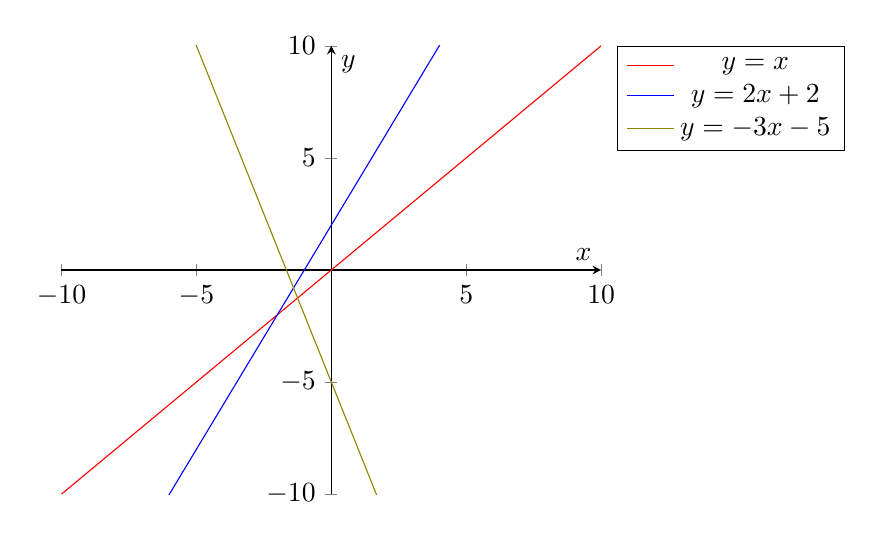
\begin{tikzpicture}
\begin{axis}[
    legend pos=outer north east,
    axis lines = left,
    axis x line = center,
    axis y line = center,
    xmin = -10,
    xmax = 10,
    ymin = -10,
    ymax = 10,
    xlabel = \(x\),
    ylabel = {\(y\)},
]
\addplot [
    domain=-10:10, 
    samples=100, 
    color=red,
]
{x};
\addlegendentry{\(y = x\)}
\addplot [
    domain=-10:10, 
    samples=100, 
    color=blue,
    ]
    {2*x + 2};
\addlegendentry{\(y = 2x + 2\)}
\addplot [
    domain=-10:10, 
    samples=100, 
    color=olive,
    ]
    {-3*x - 5};
\addlegendentry{\(y = -3x - 5\)}
\end{axis}
\end{tikzpicture}
\end{figure}

Since any flavor of Optimality Theory requires a conflict between constraints, and since \textsc{*Int Arg} is the one constraint to conflict with all the others in this account of object drop, Medina's model defines a linear function for the pairwise ordering of \textsc{*Int Arg} with respect to \textsc{Faith Arg} (\refeq{medinafunction_f}), \textsc{Telic End} (\refeq{medinafunction_t}), and \textsc{Perf Coda} (\refeq{medinafunction_p}), for a total of three different linear functions. In general, each function takes the form in \refeq{medinafunction_ex}, where the probability of \textsc{*Int Arg} being ranked above another constraint is $y$, $SPS_i$ is \alert{$x$}, $\frac{\delta_k - \gamma_k}{SPS_{max} - SPS_{min}}$ is \alert{$m$}, $\gamma_k - SPS_{min} (\frac{\delta_k - \gamma_k}{SPS_{max} - SPS_{min}})$ is \alert{$q$}, and $\delta_k$ and $\gamma_k$ are, respectively, the values the function assumes at $SPS_{max}$ and $SPS_{min}$.

\begin{equation} \labeq{medinafunction_ex}
p(\textsc{*Int Arg} \gg \textrm{con}) = \frac{\delta_k - \gamma_k}{SPS_{max} - SPS_{min}} \cdot ({SPS_{i} - SPS_{min}}) + \gamma_k
\end{equation}

In particular, the three linear functions at play are:

\begin{equation} \labeq{medinafunction_f}
p(\textsc{*Int Arg} \gg \textsc{Faith Arg}) = \frac{\delta_1 - \gamma_1}{SPS_{max} - SPS_{min}} \cdot ({SPS_{i} - SPS_{min}}) + \gamma_1
\end{equation}

\begin{equation} \labeq{medinafunction_t}
p(\textsc{*Int Arg} \gg \textsc{Telic End}) = \frac{\delta_2 - \gamma_2}{SPS_{max} - SPS_{min}} \cdot ({SPS_{i} - SPS_{min}}) + \gamma_2
\end{equation}

\begin{equation} \labeq{medinafunction_p}
p(\textsc{*Int Arg} \gg \textsc{Perf Coda}) = \frac{\delta_3 - \gamma_3}{SPS_{max} - SPS_{min}} \cdot ({SPS_{i} - SPS_{min}}) + \gamma_3
\end{equation}

These functions take positive values in a range of possible values depending on the verbs' semantic selectivity. Moreover, since the slope of each function results from the ratio between two positive-resulting differences (i.e. maximum minus minimum $y$ and $x$ values), the functions take values that are directly proportional to the verbs' Selectional Preference Strength.

\paragraph{Logical step 2: relative probabilities of the 4 constraint re-rankings} Taking a step backwards to the beginning of this Section, it was observed that four constraints result in 24 possible re-ranking orders (in \reftab{medina_24rankings}), and that this large set of permutations actually shrinks down to just four possible re-rankings if one only cares for the relative position of \textsc{*Int Arg}. In fact, the model will favor an implicit object output whenever \textsc{*Int Arg} is ranked above all the relevant constraints, regardless of their order with respect to one another. A telic perfective input only results in an implicit object output when \textsc{*Int Arg} is ranked above the three other constraints, a telic imperfective input when \textsc{*Int Arg} is ranked above \textsc{Faith Arg} and \textsc{Telic End}, an atelic perfective input when \textsc{*Int Arg} is ranked above \textsc{Faith Arg} and \textsc{Perf Coda}, and an atelic imperfective input when \textsc{*Int Arg} is ranked above \textsc{Faith Arg} alone. This results in the four possible orderings in \reftab{medina_4rankings}.

\begin{table}[htb] % the "htb" makes table env unfloaty
\caption{Set of the four possible re-rankings of \textsc{*Int Arg} with respect to \textsc{Faith Arg}, \textsc{Telic End}, and \textsc{Perf Coda}, these being unordered with respect one to another.}
\labtab{medina_4rankings} 
\begin{tabular}{|l||c|c|c|c|}\hline 
      & \vtop{\hbox{\strut \textbf{Telic}}\hbox{\strut \textbf{Perf}}}  &  \vtop{\hbox{\strut \textbf{Telic}}\hbox{\strut \textbf{Imperf}}} & \vtop{\hbox{\strut \textbf{Atelic}}\hbox{\strut \textbf{Perf}}} & \vtop{\hbox{\strut \textbf{Atelic}}\hbox{\strut \textbf{Imperf}}}\\
      \hline\hline
*I $\gg$ \{F, T, P\} & implicit  &  implicit   & implicit  & implicit \\ 
P $\gg$ *I $\gg$ \{F, T\} & overt  &  implicit   & overt  & implicit \\
T $\gg$ *I $\gg$ \{F, P\} & overt  &  overt   & implicit  & implicit \\
\{T, P\} $\gg$ *I $\gg$ F & overt  &  overt   & overt  & implicit \\\hline
\end{tabular}
\end{table}

The probability of each individual re-ranking ordering in \reftab{medina_4rankings} is equal to the joint probabilities of the independent pairwise orderings that comprise it. For instance, the probability of \textsc{*Int Arg} being ranked above all the other constraints is equal to the intersection (represented with $\cap$ in set theory) between the probability spaces of \textsc{*Int Arg} being ranked above \textsc{Faith Arg}, \textsc{*Int Arg} being ranked above \textsc{Telic End}, and \textsc{*Int Arg} being ranked above \textsc{Perf Coda}. This is rendered graphically in the Venn diagram in \reffig{venndiagram}, where the probability of \textsc{*Int Arg} being ranked above all the other constraints is colored in blue.

\begin{figure}[htb]
\caption{Graphical representation of the probability of \textsc{*Int Arg} being ranked above the three other constraints, in cyan in the Venn diagram.}
\labfig{venndiagram}
\begin{tikzpicture}
    \begin{scope}
    \clip \firstcircle;
    \clip \secondcircle;
    \fill[cyan] \thirdcircle;
    \end{scope}
\draw \firstcircle node[text=black,above] {$p(*I \gg F)$};
\draw \secondcircle node [text=black,below left] {$p(*I \gg T)$};
\draw \thirdcircle node [text=black,below right] {$p(*I \gg P)$};
    \end{tikzpicture}
    \end{figure}

In summary, the probabilities of the four rankings in \reftab{medina_4rankings} are computed as in \refeq{jointprobsmedina} to \refeq{jointprobsmedina4}. Whenever an equation features the subtraction of the probability of an event from 1, it means that the computation is taking into account the cases when that event is \textit{not} happening, given that probabilities can vary between 0 (impossible event) and 1 (certain event). For instance, since in \refeq{jointprobsmedina2} \textsc{Faith Arg} ranks above \textsc{*Int Arg}, the partial probability included in the computation is [1 - p(\textsc{*Int Arg} $\gg$ \textsc{Faith Arg})], namely the probability of \textsc{*Int Arg} \textit{not} being ranked above \textsc{Faith Arg}.

\begin{align}  \labeq{jointprobsmedina} % https://tex.stackexchange.com/questions/332430/correctly-left-align-a-set-of-equations
    & p(*I \gg {F, T, P}) = p(*I \gg F) \cdot p(*I \gg T) \cdot p(*I \gg P) \\
    & p(P \gg *I \gg {F, T}) = p(*I \gg F) \cdot p(*I \gg T) \cdot [1 - p(*I \gg P)] \labeq{jointprobsmedina2}\\
    & p(T \gg *I \gg {F, P}) = p(*I \gg F) \cdot [1 - p(*I \gg T)] \cdot p(*I \gg P) \labeq{jointprobsmedina3}\\
    & p({T, P} \gg *I \gg F) = p(*I \gg F) \cdot [1 - p(*I \gg T)] \cdot [1 - p(*I \gg P)] \labeq{jointprobsmedina4}
\end{align}

\paragraph{Logical step 3: grammaticality of implicit object output as joint probability for each aspectual type} Going back to \reftab{medina_4rankings}, the next step consists in determining the probability of an implicit object output for each of the four aspectual features in the input (the columns of the table). It is possible to achieve this result by summing the probabilities of the individual partial orderings where \textsc{*Int Arg} is ranked above the relevant constraints (the rows of the table). Thus, the likelihood of the object being dropped for each aspectual type is computed as in \refeq{aspectualprobs} to \refeq{aspectualprobs4}.

\begin{align}  \labeq{aspectualprobs}
    & p(\text{implicit})\textsubscript{Telic Perfective} = p(*I \gg {F, T, P}) \\
    & p(\text{implicit})\textsubscript{Telic Imperfective} = p(*I \gg {F, T, P}) + p(P \gg *I \gg {F, T}) \labeq{aspectualprobs2}\\
    & p(\text{implicit})\textsubscript{Atelic Perfective} = p(*I \gg {F, T, P}) + p(T \gg *I \gg {F, P}) \labeq{aspectualprobs3}\\
    & p(\text{implicit})\textsubscript{Atelic Imperfective} = p(*I \gg {F, T, P}) + p(T \gg *I \gg {F, P}) + \nonumber \\ & + p(P \gg *I \gg {F, T}) + p({T, P} \gg *I \gg F) \labeq{aspectualprobs4}
\end{align}

As stated at the beginning of this Section, in the stochastic model of the implicit object construction by \textcite{Medina2007} these probabilities indicate the gradient grammaticality of indefinite object drop for each aspectual type of input.\\
Atelic imperfective inputs violate a proper subset of the constraints violated by other aspectual types of input. Hence, also considering \reftab{medina_4rankings} and the probabilities \refeq{aspectualprobs} to \refeq{aspectualprobs4}, it is evident that the implicit object output is most likely to be grammatical with atelic imperfective inputs. Following this line of reasoning, it results that telic perfective inputs have the lowest probability to yield an implicit object output, and that the likelihood of atelic perfective and telic imperfective inputs to allow for the object to be dropped is intermediate. The relative object-dropping probability of atelic perfective inputs with respect to telic imperfective inputs depends on the parameters of the equations in \refeq{medinafunction_f}, \refeq{medinafunction_t}, and \refeq{medinafunction_p}. This state of affairs is depicted in \reffig{mock_scatter_medina}, an adaptation of the graph in \textcite[108]{Medina2007}.

\begin{figure}[htb]
\caption{Hypothetical representation of the relationship between semantic selectivity and the probability (as a proxy to grammaticality) of an implicit object output in the stochastic model by \textcite{Medina2007}. }
\labfig{mock_scatter_medina}
  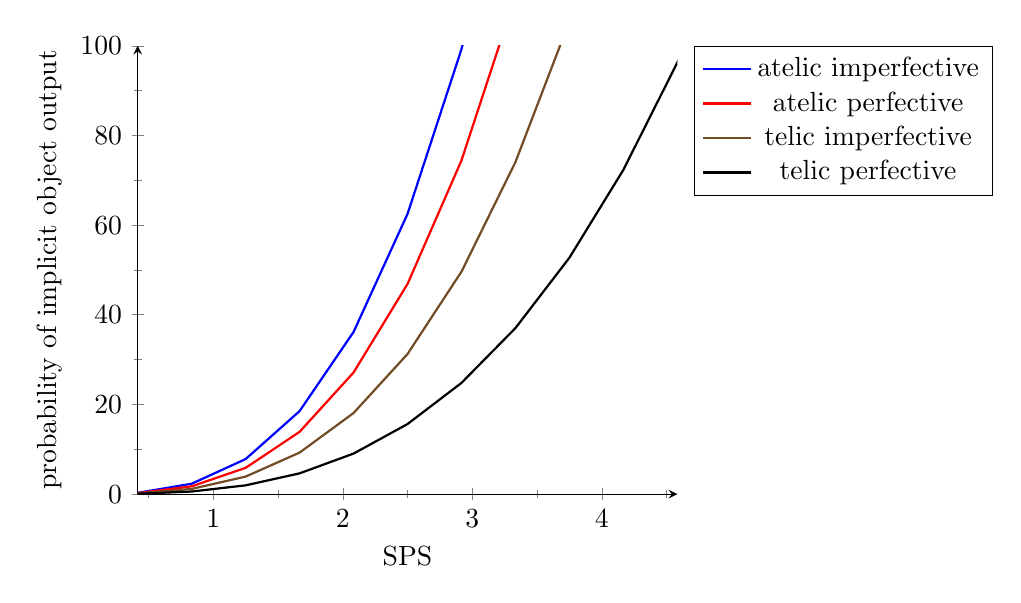
\begin{tikzpicture}
\begin{axis}[legend pos=outer north east,
    axis lines = left,scaled ticks=false,ymax=100,ymin=0,minor tick num=1,xlabel={SPS}, ylabel={probability of implicit object output}]
      \addplot+[no marks,thick] {4*(x^3)};
      \addlegendentry{atelic imperfective};
      \addplot+[no marks,thick] {3*(x^3)};
      \addlegendentry{atelic perfective};
      \addplot+[no marks,thick] {2*(x^3)};
      \addlegendentry{telic imperfective};
      \addplot+[no marks,thick] {x^3};
      \addlegendentry{telic perfective};
    \end{axis}
  \end{tikzpicture}
\end{figure}

The curves in \reffig{mock_scatter_medina} are cubic functions because the computations in  \refeq{jointprobsmedina} to \lrefeq{jointprobsmedina4} involve the multiplication of the three linear functions of the type illustrated in \refeq{medinafunction_ex}. This means that the unknown $SPS_i$ (the $x$ of the linear function) gets multiplied three times by itself, resulting in ${SPS_i}^3$, which yields a cubic curve. Of course all the parameters in the complex function in \refeq{medinafunction_ex} are part of the newly created cubic function, but they do not result in a higher grade (i.e. more than cubic) polynomial function since they are not unknowns of the function.

\subsection{Implementing a probabilistic constraint ranking} \labsec{medinacomputation}

\paragraph{Introduction} The three-step logic illustrated in \refsec{rankingmedina} is mirrored by the three-step procedure used to computationally implement the probabilistic constraint ranking. The computational steps devised by Medina are as follows:

\begin{enumerate}
    \item the grammaticality the indefinite object drop is quantified via an acceptability judgment survey, the results thereof are equated to the probability of an implicit object output for a given input
    \item the probability of each of the four possible constraint orderings can be estimated via the probability of an implicit object output
    \item knowing the probability of each constraint ordering, it's possible to estimate the probability of \textsc{*Int Arg} dominating each constraint
\end{enumerate}

As is evident from comparing the logical and computational steps (see \reftab{medina_nicetable}), the technical implementation of the model goes backwards with respect to the underlying logic.

\begin{table}[htb] % the "htb" makes table env unfloaty
\caption{Three-step design of Medina's model: computational steps mirror logical steps}
\labtab{medina_nicetable} 
\begin{tabular}{c c}
 & \\
\cmidrule{1-1} % richiede un range! else esce COMPILE TIMEOUT ERROR
\textbf{Logic} &                      \\
\textbf{$\downarrow$} &                      \\ \hline
step 1         & step 3               \\
step 2         & step 2               \\
step 3         & step 1               \\ \hline
               & \textbf{$\uparrow$} \\
               & \textbf{Computation} \\
\cmidrule{2-2}           
\end{tabular}
\end{table}

Let us discuss each computational step in more detail.

\paragraph{Computational step 1: Collecting acceptability judgments} The collection of acceptability judgments is not a part of the computational procedure \textit{per se}, unlike the estimation of the parameters of the linear functions. However, since acceptability judgments are directly equated to the probability of an implicit object output, the fine points of their collection belong to this section nonetheless. I will now present the main aspects of Medina's experimental design, which the interested reader can find and integrate with additional information in \textcite[110-134]{Medina2007}.\\
The linguistic predictors of object drop under consideration are semantic selectivity, telicity, and perfectivity. Among these, semantic selectivity and telicity are inherent properties of each verb, while perfectivity is a sentence-level property. For this reason, the verbs in the experiment are annotated with respect to their semantic selectivity and telicity, while sentences are manipulated for perfectivity. This results in a 2x2 factorial design\sidenote{A experimental design with two independent variables having two levels each, resulting in four experimental conditions.} where each verb, having its own selectivity and telicity profile, appears both with and without a direct object, and both having and lacking the perfectivity feature. The examples in \ref{medina_exstim} are adapted from \textcite[113]{Medina2007}.

\ex. \label{medina_exstim} \a. \label{medina_exstim1} Michael had brought.
\b. \label{medina_exstim2}  Michael was bringing.
\c. \label{medina_exstim3}  Sarah had brought a gift.
\d. \label{medina_exstim4}  Sarah was bringing a gift.

The telicity of each verb was deemed to be [+Telic] if two out of three tests yielded a telic interpretation, [-Telic] otherwise. As discussed in \refsec{predictor_telicity} in regards to the telicity tests of choice in my own model, there is something to be said about the feasibility of this particular set of tests. However, they yielded very consistent results, and henceforth they cannot be considered as a crack in the otherwise very solid foundation of Medina's design. The three tests \parencite[302-303]{Medina2007} are:
\begin{itemize}
    \item \textbf{The \textit{almost} test.} Predicates marked as [+Telic] and appearing with the adverb \textit{almost} (e.g. \textit{Tony almost packed.} can be interpreted as describing either an event that has begun but has not finished, or an event that has not yet begun. On the contrary, [-Telic] predicates with \textit{almost} (e.g. \textit{Tony almost ate.}) can only get the second interpretation.
    \item \textbf{The \textit{in/for} test.} [+Telic] predicates are more natural with \textit{in X time} as an adjunct (e.g. \textit{Michelle made some stuff in/*for five minutes.}), while [-Telic] ones prefer \textit{for X time} (e.g. \textit{Michelle read *in/for five minutes.}).
    \item \textbf{The \textit{counting} test.} Counting a [+Telic] predicate results in a natural interpretation where it denotes multiple, separate events (e.g. \textit{Edgar opened some stuff three times.}), while counted [-Telic] predicates appear as if denoting multiple instances of the same event (e.g. \textit{Edgar watched some stuff three times.}).
\end{itemize}

Using a set of 30 transitive verbs of interest and 10 intransitive verbs resulted in a set of 160 sentences to be used as experimental stimuli (because of the 2x2 design). The 30 transitive verbs were the same used by \textcite{Resnik1993, Resnik1996} to test his Selectional Preference Strength, since \textcite{Medina2007} employs the same measure to quantify semantic selectivity. Of the 160 stimuli, the 40 intransitive sentences were used as fillers to distract the participants from the real focus of the experiment, the 60 transitive sentences with an overt object were used as controls (since they had to be grammatical by default), and the remaining 60 transitive sentences \textit{without} a direct object were the actual target of the experiment.\\
A total of 15 native speakers of English were recruited as participants among the undergraduate students of Johns Hopkins University and rewarded class credit for their effort. Each of them saw all the stimuli in every experimental condition in randomized order, i.e. the experiment followed a within-subject crossed design. Participants partook in a short training session with 3 mock stimuli before accessing the experiment proper, and received immediate feedback. Both in the training session and the experimental session, participants had to score each stimulus on a 5-point Likert scale ranging from 1 (ungrammatical) to 5 (fully grammatical).

\paragraph{Computational step 2: Judgments and probabilities} The acceptability judgments thus obtained for each verb in each experimental condition were considered equal to the probability of the implicit object output to be returned by the stochastic model based on all the possible re-rankings of the constraints at play for that given input. The judgment scores were then used to estimate the probabilities of the four possible constraint rankings in \reftab{medina_4rankings}, which in turn were used to estimate the probabilities of \textsc{*Int Arg} dominating each of the other three constraints. Let us retrace the computational steps that lead to this result.\\
As shown before, the probability of an implicit object output for each aspectual type of input is equal to the joint probability of the independent pairwise rankings of the relevant constraints. This is shown in \refeq{aspectualprobs} to \refeq{aspectualprobs4}, reported here again for ease of consultation.

\begin{align*}  \tag{\refeq{aspectualprobs}}
    & p(\text{implicit})\textsubscript{Telic Perfective} = p(*I \gg {F, T, P}) \\
    & p(\text{implicit})\textsubscript{Telic Imperfective} = p(*I \gg {F, T, P}) + p(P \gg *I \gg {F, T}) \tag{\refeq{aspectualprobs2}}\\
    & p(\text{implicit})\textsubscript{Atelic Perfective} = p(*I \gg {F, T, P}) + p(T \gg *I \gg {F, P}) \tag{\refeq{aspectualprobs3}}\\
    & p(\text{implicit})\textsubscript{Atelic Imperfective} = p(*I \gg {F, T, P}) + p(T \gg *I \gg {F, P}) + \nonumber \\ & + p(P \gg *I \gg {F, T}) + p({T, P} \gg *I \gg F) \tag{\refeq{aspectualprobs4}}
\end{align*}

Based on the calculations in \refeq{jointprobsmedina} to \refeq{jointprobsmedina4}, the aforementioned joint probabilities are computed as follows in \refeq{jointcomplete} to \refeq{jointcomplete4}.

\begin{align}  \labeq{jointcomplete}
    & p(\text{implicit})\textsubscript{Telic Perfective} = p(*I \gg F) \cdot p(*I \gg T) \cdot p(*I \gg P) \\
    & p(\text{implicit})\textsubscript{Telic Imperfective} = p(*I \gg F) \cdot p(*I \gg T) \cdot p(*I \gg P) + \nonumber \\ & + p(*I \gg F) \cdot p(*I \gg T) \cdot [1 - p(*I \gg P)] \labeq{jointcomplete2}\\
    & p(\text{implicit})\textsubscript{Atelic Perfective} = p(*I \gg F) \cdot p(*I \gg T) \cdot p(*I \gg P) + \nonumber \\ & + p(*I \gg F) \cdot [1 - p(*I \gg T)] \cdot p(*I \gg P) \labeq{jointcomplete3}\\
    & p(\text{implicit})\textsubscript{Atelic Imperfective} = p(*I \gg F) \cdot p(*I \gg T) \cdot p(*I \gg P) + \nonumber \\ & + p(*I \gg F) \cdot [1 - p(*I \gg T)] \cdot p(*I \gg P) + \nonumber \\ & + p(*I \gg F) \cdot p(*I \gg T) \cdot [1 - p(*I \gg P)] + \nonumber \\ & + p(*I \gg F) \cdot [1 - p(*I \gg T)] \cdot [1 - p(*I \gg P)] \labeq{jointcomplete4}
\end{align}

\paragraph{Computational step 3: Parameter estimation} The last step involves \refeq{medinafunction_f}, \refeq{medinafunction_t}, and \refeq{medinafunction_p}, where the ranking of \textsc{*Int Arg} with respect to the other three constraints was defined as a (linear) function of the input verb's semantic selectivity. Plugging them in \refeq{jointcomplete} results in the (cubic) function in \refeq{cubic_telperf}, describing the probability of an implicit object output with a telic perfective input depending on the specific verb's semantic selectivity.

\begin{align}  \labeq{cubic_telperf}
    & p(\text{implicit})\textsubscript{Telic Perfective} = [\frac{\delta_1 - \gamma_1}{SPS_{max} - SPS_{min}} \cdot ({SPS_{i} - SPS_{min}}) + \gamma_1] \cdot \nonumber \\ & \cdot [\frac{\delta_2 - \gamma_2}{SPS_{max} - SPS_{min}} \cdot ({SPS_{i} - SPS_{min}}) + \gamma_2] \cdot \nonumber \\ & \cdot [\frac{\delta_3 - \gamma_3}{SPS_{max} - SPS_{min}} \cdot ({SPS_{i} - SPS_{min}}) + \gamma_3]
\end{align}

The value of the function, i.e. $p(\text{implicit})\textsubscript{Telic Perfective}$, is the average acceptability judgment for a telic perfective input with a known SPS, i.e. $SPS_{i}$ in the equation. The values of $SPS_{max}$ and $SPS_{min}$ are known, since they are the maximum and minimum Selectional Preference Strength values in Resnik's list, respectively. Henceforth, the equation has only to be solved for $\delta_i$ and $\gamma_i$, which are the values the function takes at $SPS_{max}$ and $SPS_{min}$ respectively. A similar reasoning applies to telic imperfective, atelic perfective, and atelic imperfective inputs, once again plugging \refeq{medinafunction_f}, \refeq{medinafunction_t}, and \refeq{medinafunction_p} into \refeq{jointcomplete2}, \refeq{jointcomplete3}, and \refeq{jointcomplete4}.\\
At the end of this process, the experimenter is left with a set of $n$ equations, each having six unknowns to be solved for, where $n$ is the total number of target sentences among the stimuli. In order to calculate $\delta_i$ and $\gamma_i$, the judgments (i.e. the probabilities of object drop which serve as values of the functions) underwent two preprocessing steps in Medina's pipeline, namely:
\begin{enumerate}
    \item for each target sentence, the 15 judgments provided by 15 participants were averaged into a single numerical value, and
    \item this numerical value was converted linearly to fall between 0 and 1, since this is the proper range for probabilities
\end{enumerate}

Medina estimated the values of the unknown parameters using Excel Solver\sidenote{An add-in component of Microsoft Excel used to find the optimal value of a function based on several constraints.}, based on the following two constraints:
\begin{itemize}
    \item $\delta_i$ and $\gamma_i$ have to fall between 0 and 1
    \item the sum-squared error between the predictions of the model and the actual grammaticality judgment data have to be minimized
\end{itemize}
Thanks to these constraints, the model outputs predicted grammaticality values in the 0-1 probability range.

\paragraph{Summary of results} The values of $\delta_i$ and $\gamma_i$ Medina found as a result of this optimization indicate that in English, \textsc{*Int Arg} is more likely to dominate each of the other three constraints when the verb is highly semantically selective, and this is most evident for \textsc{Telic End}. The actual values are

FARE TABELLA CON DUE COLONNE PER DELTA E GAMMA E NOMINARE CIASCUNA RIGA CON P(INTARG << CONSTRAINT)

These results are visualized in \reffig{medina_intargabove}, adapted from \textcite[143-144]{Medina2007}.

\begin{figure}[htb]
\caption{DIDASCALIA.}
\labfig{medina_intargabove}
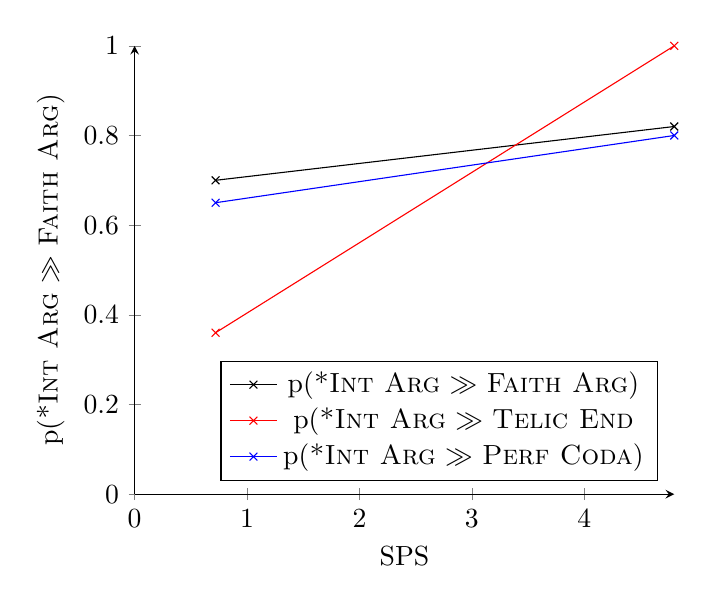
\begin{tikzpicture}
    \begin{axis}[legend pos=south east, xmin=0, ymin=0, ymax=1, axis lines = left,scaled ticks=false, xlabel={SPS}, ylabel={p(\textsc{*Int Arg} $\gg$ \textsc{Faith Arg})}] 
        \addplot[color=black,mark=x] coordinates {
        (0.72,0.70) 
        (4.80,0.82) 
    }; 
      \addlegendentry{p(\textsc{*Int Arg} $\gg$ \textsc{Faith Arg})};
            \addplot[color=red,mark=x] coordinates {
        (0.72,0.36) 
        (4.80,1.00) 
    }; 
    \addlegendentry{p(\textsc{*Int Arg} $\gg$ \textsc{Telic End}};
            \addplot[color=blue,mark=x] coordinates {
        (0.72,0.65) 
        (4.80,0.80) 
    }; 
    \addlegendentry{p(\textsc{*Int Arg} $\gg$ \textsc{Perf Coda})};
    % \node [above] at (axis cs:  0.72,0.70) {(0.72,0.70)};
    % \node [above left] at (axis cs:  4.80,0.82) {(4.80,0.82)};
    \end{axis} 
\end{tikzpicture}
\end{figure}

testo testo testo

GRAFICO CON LE 4 FUNZIONI TUTTE INSIEME (plottare punto per punto), cfr \reffig{mock_scatter_medina}

% \begin{figure}[htb]
% \caption{Hypothetical representation of the relationship between semantic selectivity and the probability (as a proxy to grammaticality) of an implicit object output in the stochastic model by \textcite{Medina2007}. }
% \labfig{mock_scatter_medina}
%   \begin{tikzpicture}
% \begin{axis}[legend pos=outer north east,
%     axis lines = left,scaled ticks=false,ymax=100,ymin=0,minor tick num=1,xlabel={SPS}, ylabel={probability of implicit object output}]
%       \addplot+[no marks,thick] {4*(x^3)};
%       \addlegendentry{atelic imperfective};
%       \addplot+[no marks,thick] {3*(x^3)};
%       \addlegendentry{atelic perfective};
%       \addplot+[no marks,thick] {2*(x^3)};
%       \addlegendentry{telic imperfective};
%       \addplot+[no marks,thick] {x^3};
%       \addlegendentry{telic perfective};
%     \end{axis}
%   \end{tikzpicture}
% \end{figure}




\section{Building on Medina TOGLIERE E ACCORPARE AL PROSSIMO CAPITOLO} \labsec{improvingmedina}

Improving the original model (aggiungere sezione/paragrafo sul fatto che il mio modello computazionale è in Python, più scalabile se faccio alcune opportune modifiche, e tratta meglio le variabili (vedere se medina normalizza i dati, etc))


\subsection{Semantic selectivity} \labsec{pisasps}

spostare qui il paragrafo su PISA che adesso sta in predictors.tex


\subsection{More constraints} \labsec{newconstraints}

text

% \alert{Iterativity} and \alert{manner specification} (\hyperlink{otherfactors}{\beamergotobutton{back to origins}}) can become two markedness constraints based on binary features of the predicate ([+/- iterative, +/- specified]):
% \begin{itemize}
    % \item \textsc{Non-Iterative Argument (Non-Iter Arg)}: non-iterative predicates must occur with an overt argument in the output
    % \item \textsc{Manner-Specified Argument (Man-Spec Arg)}: manner-specified predicates must occur with an overt argument in the output
% \end{itemize}
% {\small As with \textsc{Telic End} and \textsc{Perf Coda}, \textbf{the omission of a dObj} violates them} \\~\\
% {\footnotesize The experimental design will accomodate them easily: \hyperlink{expsetting}{\beamergotobutton{Experimental setting}}}


\subsection{Crosslinguistic evidence} \labsec{crossling}

text

% Literature agrees on the lack of \alert{cross-linguistic accounts} of argument omissibility, so it would be super interesting to be among the pioneers! Comparing the results of my model and seeing whether there is some pattern in the way verbs cluster cross-linguistically with respect to the omissibility of their objects/Instruments is something I would really like to do.\\~\\ {\small The experimental design and my Python scripts are easily \alert{adaptable} to this purpose, and I can create both data/stimuli-sets.}


\subsection{Open Science paradigm} \labsec{sharingiscaring}

text

% I estimated Medina's parameters using \alert{Python}. Following Paul's suggestion (thanks!) I looked into library optimization functions that find minima of functions and finally chose \alert{scipy.optimize.curve\_fit} among the many available.\\~\\
% My script also computes \alert{everything else}: Medina's original model, the partially extended model, the full extended model, data exploration and preprocessing, model evaluations, and figures.\\~\\
% If you are interested, the script(s) and mock input data are \href{https://github.com/giuliacappelli/MedinaStochasticOptimalityTheory}{\textbf{here}} on my \alert{GitHub} profile with a detailed explanation.